\documentclass[11pt]{article}

\usepackage[utf8]{inputenc}
\usepackage[T1]{fontenc}
\usepackage{amsmath,amssymb}
\usepackage{graphicx}
\usepackage{booktabs}
\usepackage{hyperref}
\usepackage[margin=1in]{geometry}
\usepackage{caption}
\usepackage{subcaption}

\graphicspath{{paper_figs/}}

\title{Hallazgos: Pooled Testing Dinamico con Tests Aumentados (DAPTS)}
\author{}
\date{}

\begin{document}

\maketitle

\begin{abstract}
Probamos grupos de personas en vez de una por una.
Nuestros tests son ``aumentados'': en vez de solo decir positivo/negativo,
dicen \emph{cuantos} infectados hay en el grupo.
Con esa informacion extra, decidimos mejor que testear despues.

Tres resultados principales:
(1) Existe una cadena de estrategias donde cada una es mejor que la anterior.
(2) La ventaja del test aumentado es mayor con grupos mas grandes y presupuesto intermedio.
(3) La estrategia es robusta: funciona bien aunque no conozcamos las probabilidades exactas.
\end{abstract}

%% ====================================================================
\section{Cadena de Estrategias}
\label{sec:chain}

Comparamos 6 estrategias, de peor a mejor:

\begin{equation}
  U_{\text{single}} \leq U^s_{\text{NO}} \leq U^s_O \leq U^D \leq U^D_A \leq U_{\max}
  \label{eq:chain}
\end{equation}

Que significa cada una:
\begin{itemize}
  \item $U_{\text{single}}$: testear personas una por una
  \item $U^s_{\text{NO}}$: grupos fijos, sin traslape
  \item $U^s_O$: grupos fijos, con traslape
  \item $U^D$: grupos adaptativos (binario: positivo/negativo)
  \item $U^D_A$: grupos adaptativos + test aumentado (cuenta cuantos infectados)
  \item $U_{\max}$: cota superior teorica (si supieramos todo)
\end{itemize}

La ganancia total $U_{\max} - U_{\text{single}}$ se descompone en 4 partes:
\textbf{agrupar} ($U^s_{\text{NO}} - U_{\text{single}}$),
\textbf{traslapar} ($U^s_O - U^s_{\text{NO}}$),
\textbf{adaptar} ($U^D - U^s_O$), y
\textbf{aumentar} ($U^D_A - U^D$).

Probado con $n \in \{4,5,6\}$, $B \in \{2,3\}$, $G = 3$, 10 instancias aleatorias por configuracion.

\begin{figure}[htbp]
  \centering
  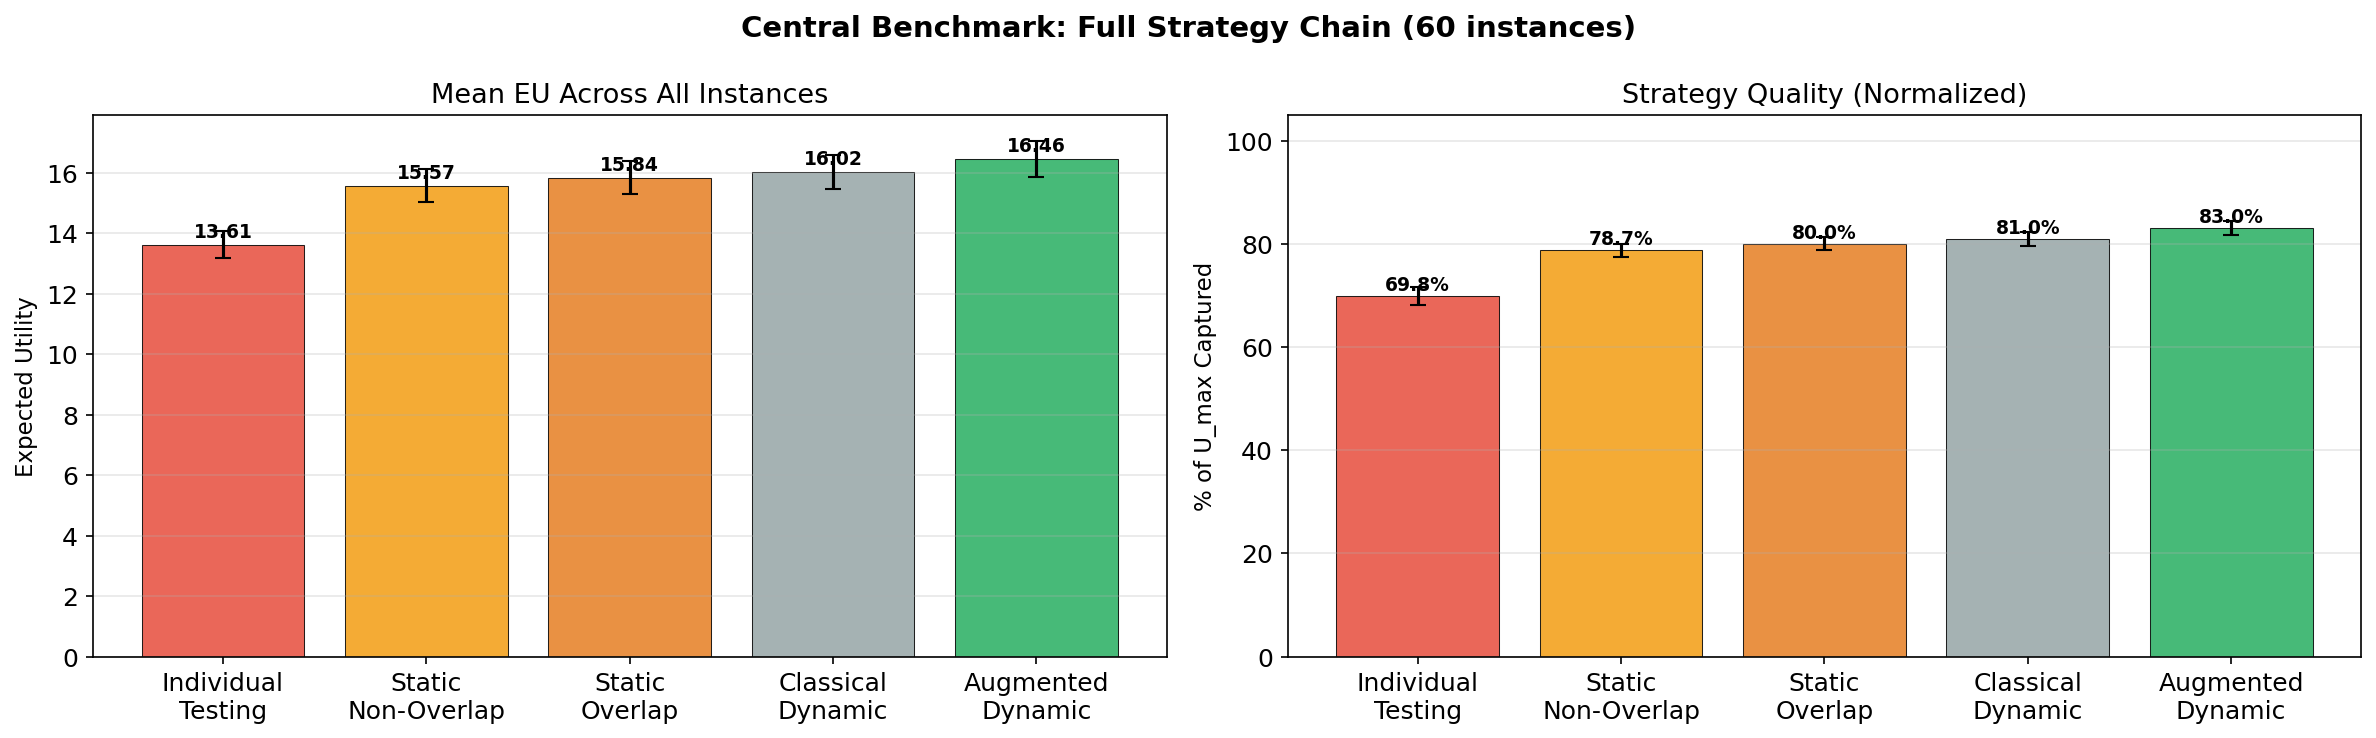
\includegraphics[width=0.85\textwidth]{central_benchmark_chain.png}
  \caption{La cadena se cumple en todas las instancias.}
  \label{fig:chain}
\end{figure}

\begin{figure}[htbp]
  \centering
  \begin{subfigure}[t]{0.48\textwidth}
    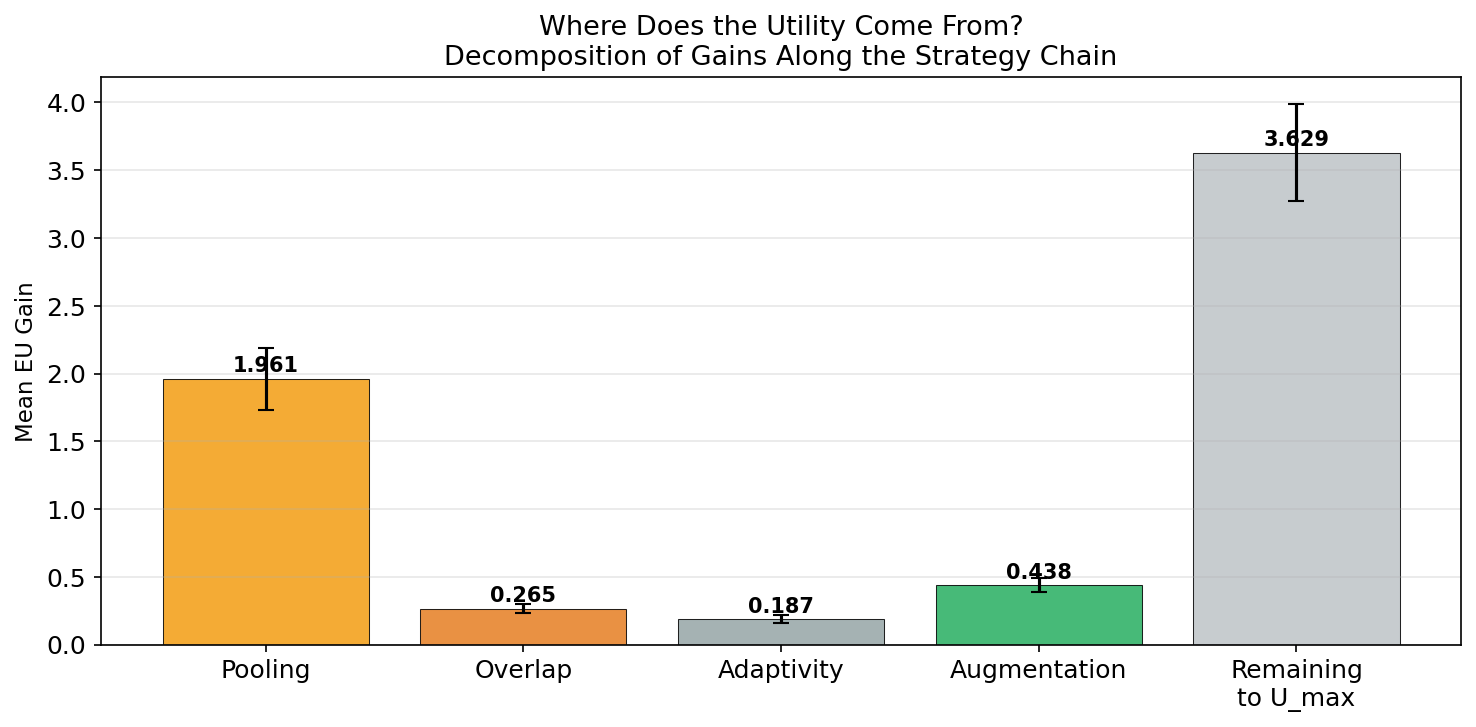
\includegraphics[width=\textwidth]{gain_decomposition.png}
    \caption{Descomposicion de ganancias.}
  \end{subfigure}
  \hfill
  \begin{subfigure}[t]{0.48\textwidth}
    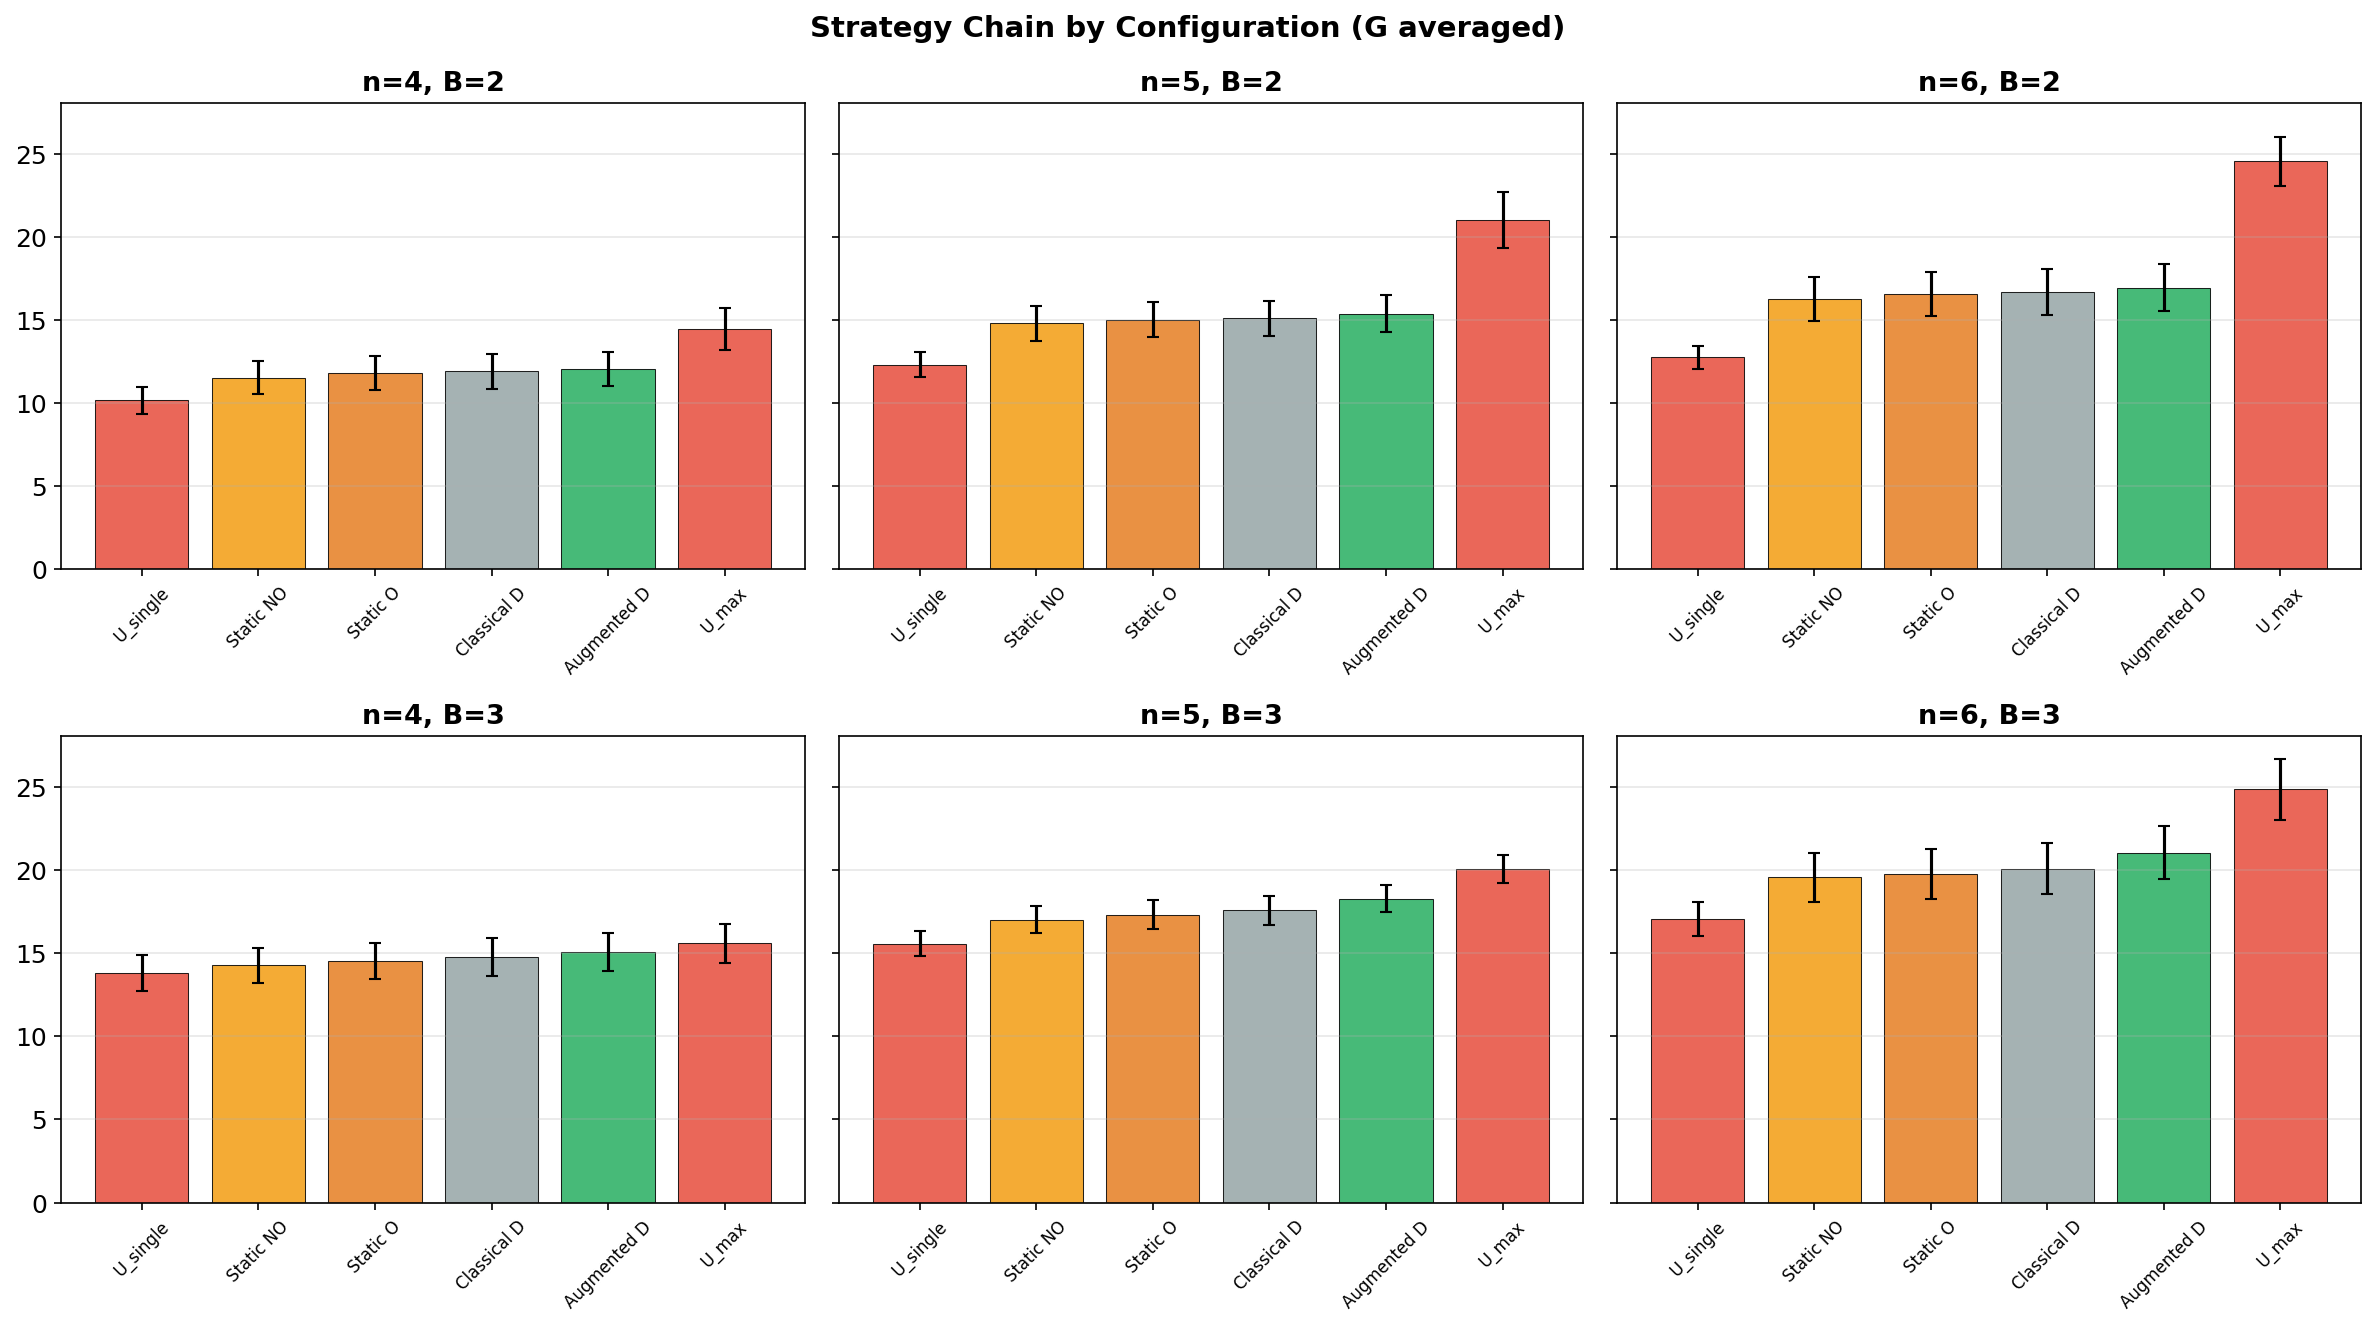
\includegraphics[width=\textwidth]{strategy_chain_by_config.png}
    \caption{Cadena por configuracion $(n, B)$.}
  \end{subfigure}
  \caption{Cada fuente de ganancia contribuye algo distinto.}
\end{figure}

%% ====================================================================
\section{Cuando Ayuda el Test Aumentado?}
\label{sec:regime}

Dos experimentos:

\textbf{Mapa de regimen.} Variamos prevalencia (5\%--70\%) y tamano maximo de grupo $G$ (2--5), con $n=5$, $B=3$, 10 instancias.
El test aumentado ayuda mas con prevalencia moderada-alta y grupos grandes.
Con $G=1$ (tests individuales), aumentado = clasico.

\textbf{Barrido de $G$.} Con 8 instancias pareadas ($n=6$, $B=3$, $G=1\ldots6$), comparamos todas las estrategias.
El aumentado se beneficia mas que las demas al crecer $G$, porque grupos mas grandes generan conteos mas informativos.

\begin{figure}[htbp]
  \centering
  \begin{subfigure}[t]{0.48\textwidth}
    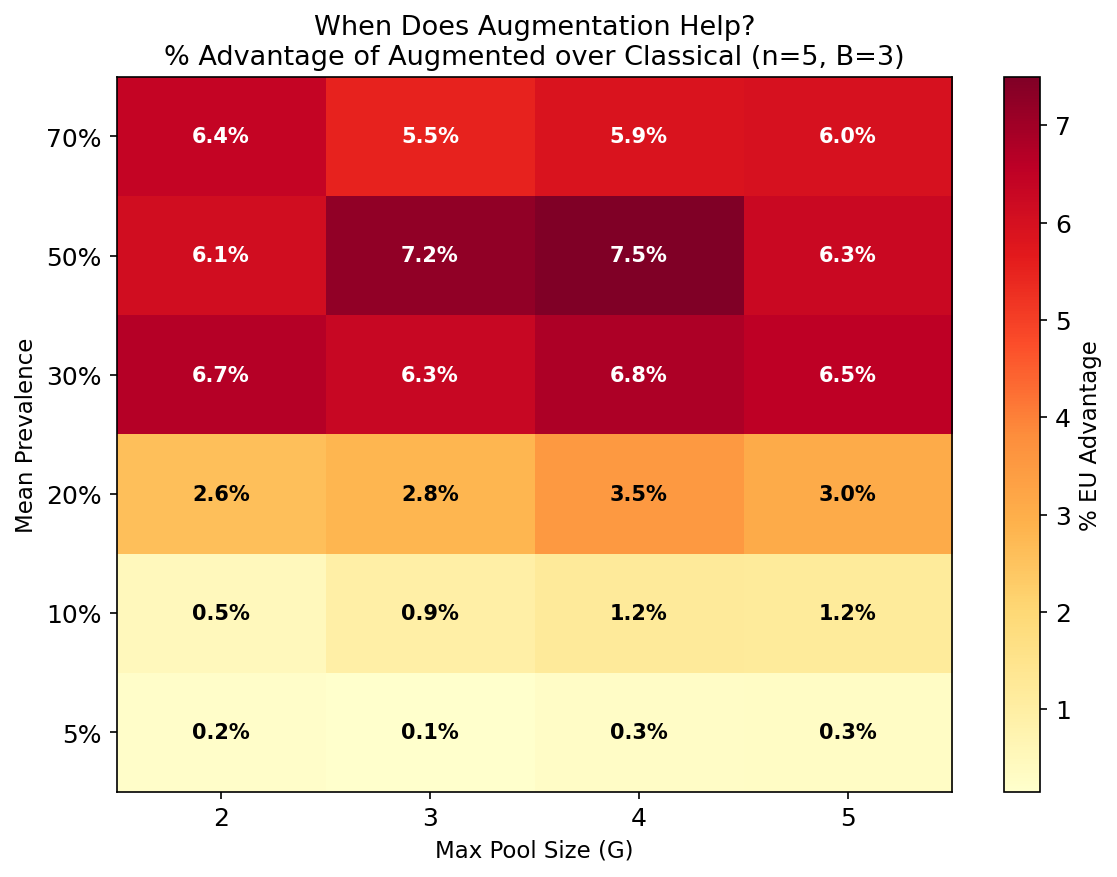
\includegraphics[width=\textwidth]{regime_map_augmentation.png}
    \caption{Mapa: ventaja por prevalencia y $G$.}
  \end{subfigure}
  \hfill
  \begin{subfigure}[t]{0.48\textwidth}
    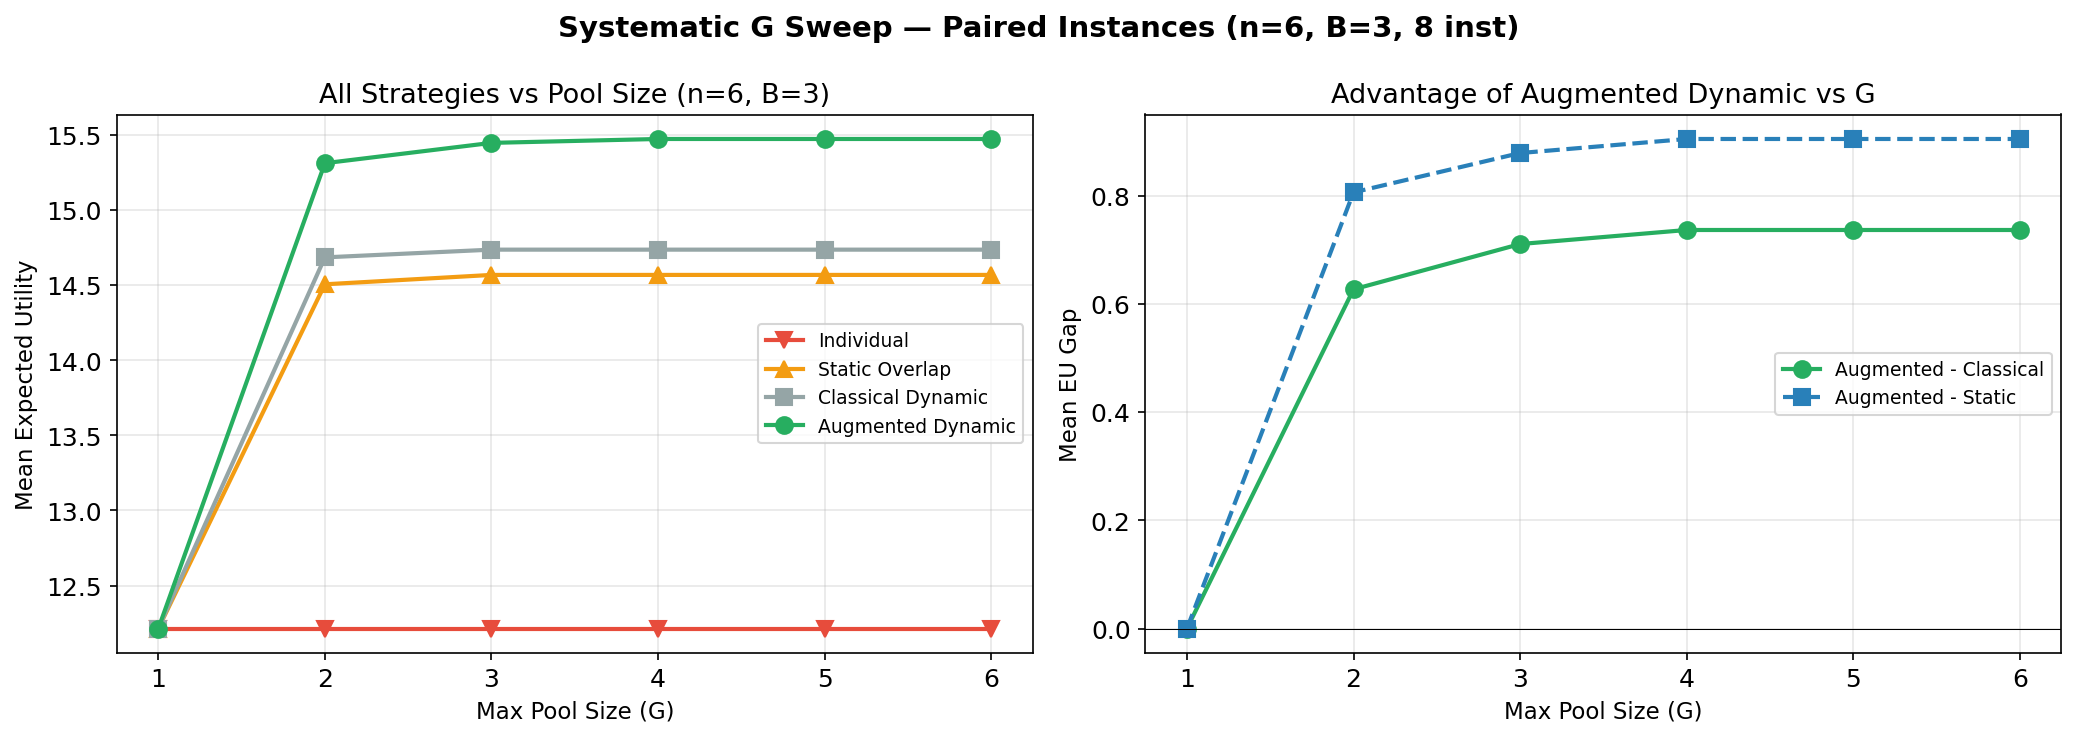
\includegraphics[width=\textwidth]{g_sweep_all_strategies.png}
    \caption{Todas las estrategias vs $G$.}
  \end{subfigure}
  \caption{El test aumentado ayuda mas con prevalencia alta y grupos grandes.}
\end{figure}

%% ====================================================================
\section{Efecto del Presupuesto de Tests}
\label{sec:budget}

Variamos el presupuesto $B = 1\ldots6$ con $n=6$, $G=3$, 8 instancias pareadas.

\textbf{Resultado:} la ventaja del aumentado es mayor a $B$ intermedio.
A $B$ grande (cercano a $n$), todos los individuos se resuelven y la ventaja desaparece.

Con poblacion heterogenea (2 VIPs con $u=10$, 4 comunes con $u=1$), la ventaja es aun mayor.

\begin{figure}[htbp]
  \centering
  \begin{subfigure}[t]{0.48\textwidth}
    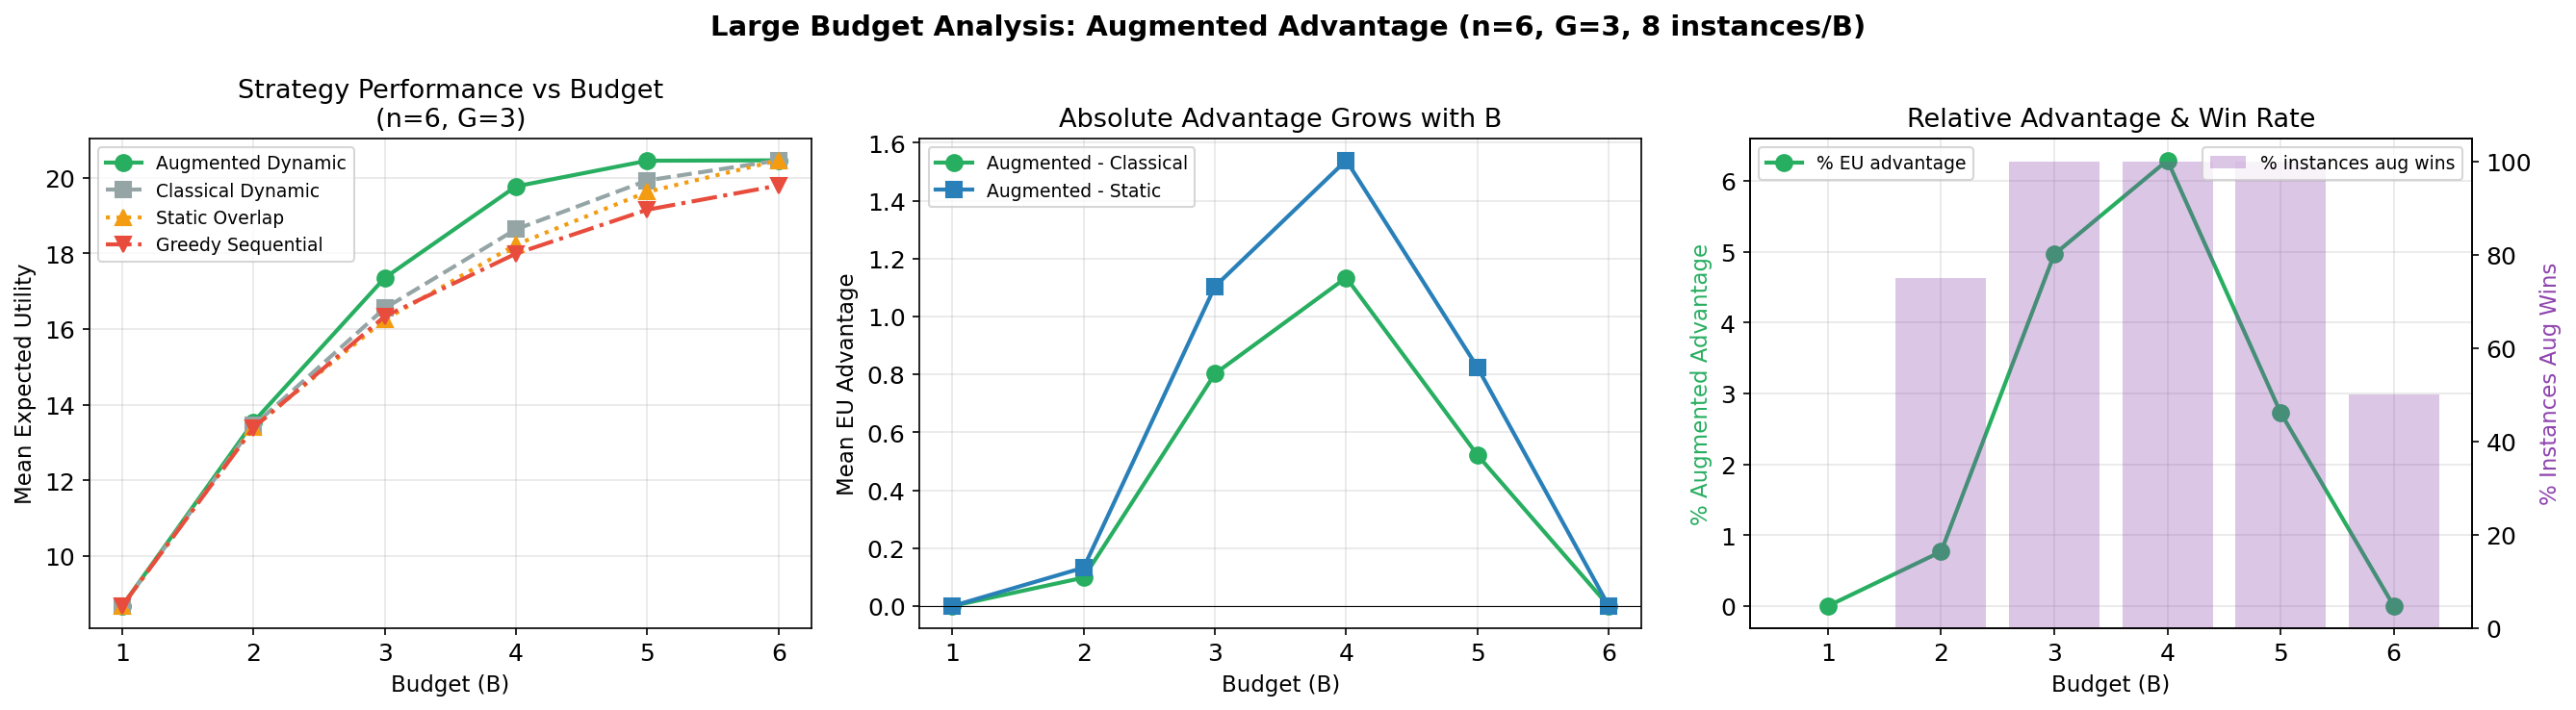
\includegraphics[width=\textwidth]{large_budget_advantage.png}
    \caption{Ventaja vs $B$ (pico a $B$ intermedio).}
  \end{subfigure}
  \hfill
  \begin{subfigure}[t]{0.48\textwidth}
    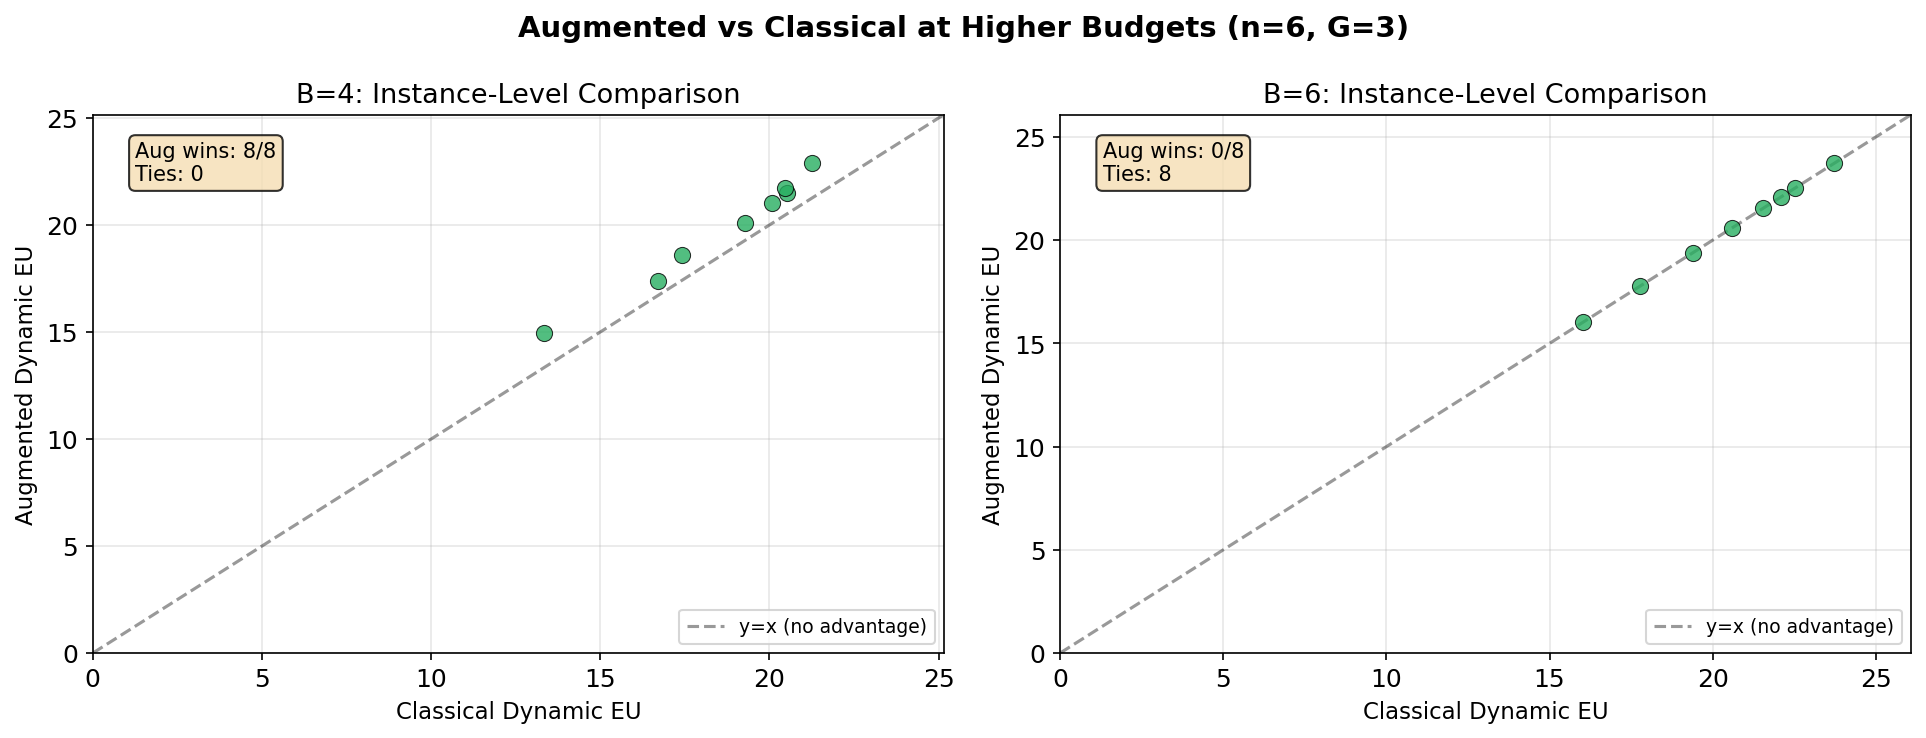
\includegraphics[width=\textwidth]{large_b_scatter.png}
    \caption{Aumentado vs clasico, instancia por instancia.}
  \end{subfigure}
\end{figure}

\begin{figure}[htbp]
  \centering
  \begin{subfigure}[t]{0.48\textwidth}
    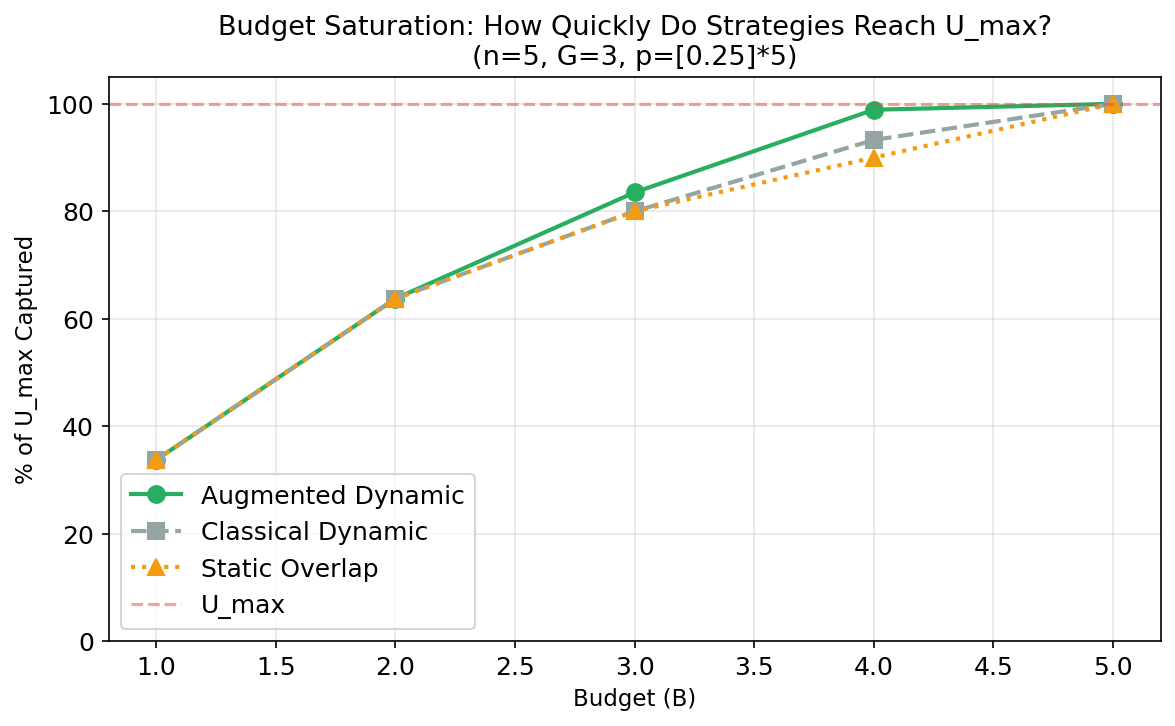
\includegraphics[width=\textwidth]{budget_saturation.png}
    \caption{Saturacion (poblacion homogenea).}
  \end{subfigure}
  \hfill
  \begin{subfigure}[t]{0.48\textwidth}
    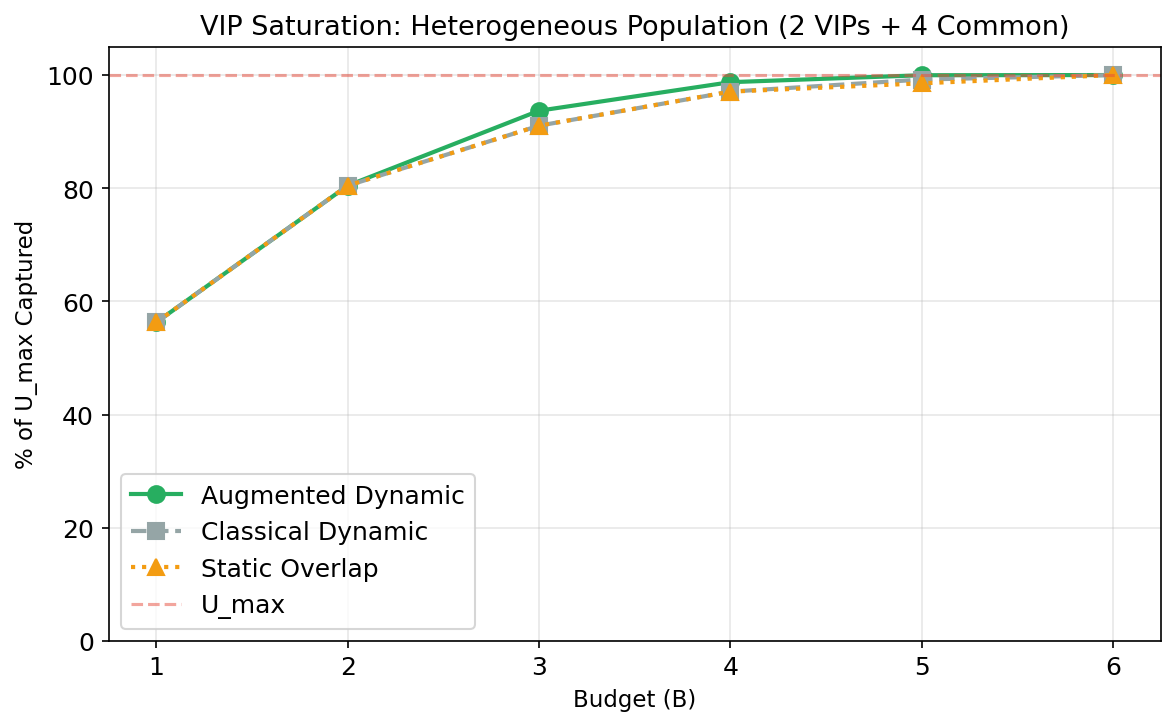
\includegraphics[width=\textwidth]{vip_budget_saturation.png}
    \caption{Saturacion (poblacion VIP).}
  \end{subfigure}
  \caption{Con mas tests, todas las estrategias se acercan a $U_{\max}$, pero el aumentado llega primero.}
\end{figure}

%% ====================================================================
\section{Informacion Cruzada: El Mecanismo Clave}
\label{sec:crosstest}

Por que funciona mejor el test aumentado? Por la \textbf{informacion cruzada entre tests}.

El conteo exacto de un test actualiza las creencias sobre personas en \emph{otros} tests.
El test binario (positivo/negativo) no puede hacer esto tan bien.

Para medirlo, comparamos 3 enfoques:
\begin{itemize}
  \item \textbf{Greedy secuencial}: actualiza creencias test por test (ignora correlaciones).
  \item \textbf{Greedy counting}: actualiza con toda la historia (captura correlaciones).
  \item \textbf{Optimo DP}: solucion exacta.
\end{itemize}

La diferencia counting $-$ secuencial = valor de la informacion cruzada.
Este valor es mayor a $B$ intermedio. A $B$ grande, ambos convergen porque la mayoria de individuos ya estan resueltos.

Probado con $n=6$, $G=3$, $B \in \{2,\ldots,5\}$, 8 instancias pareadas.

\begin{figure}[htbp]
  \centering
  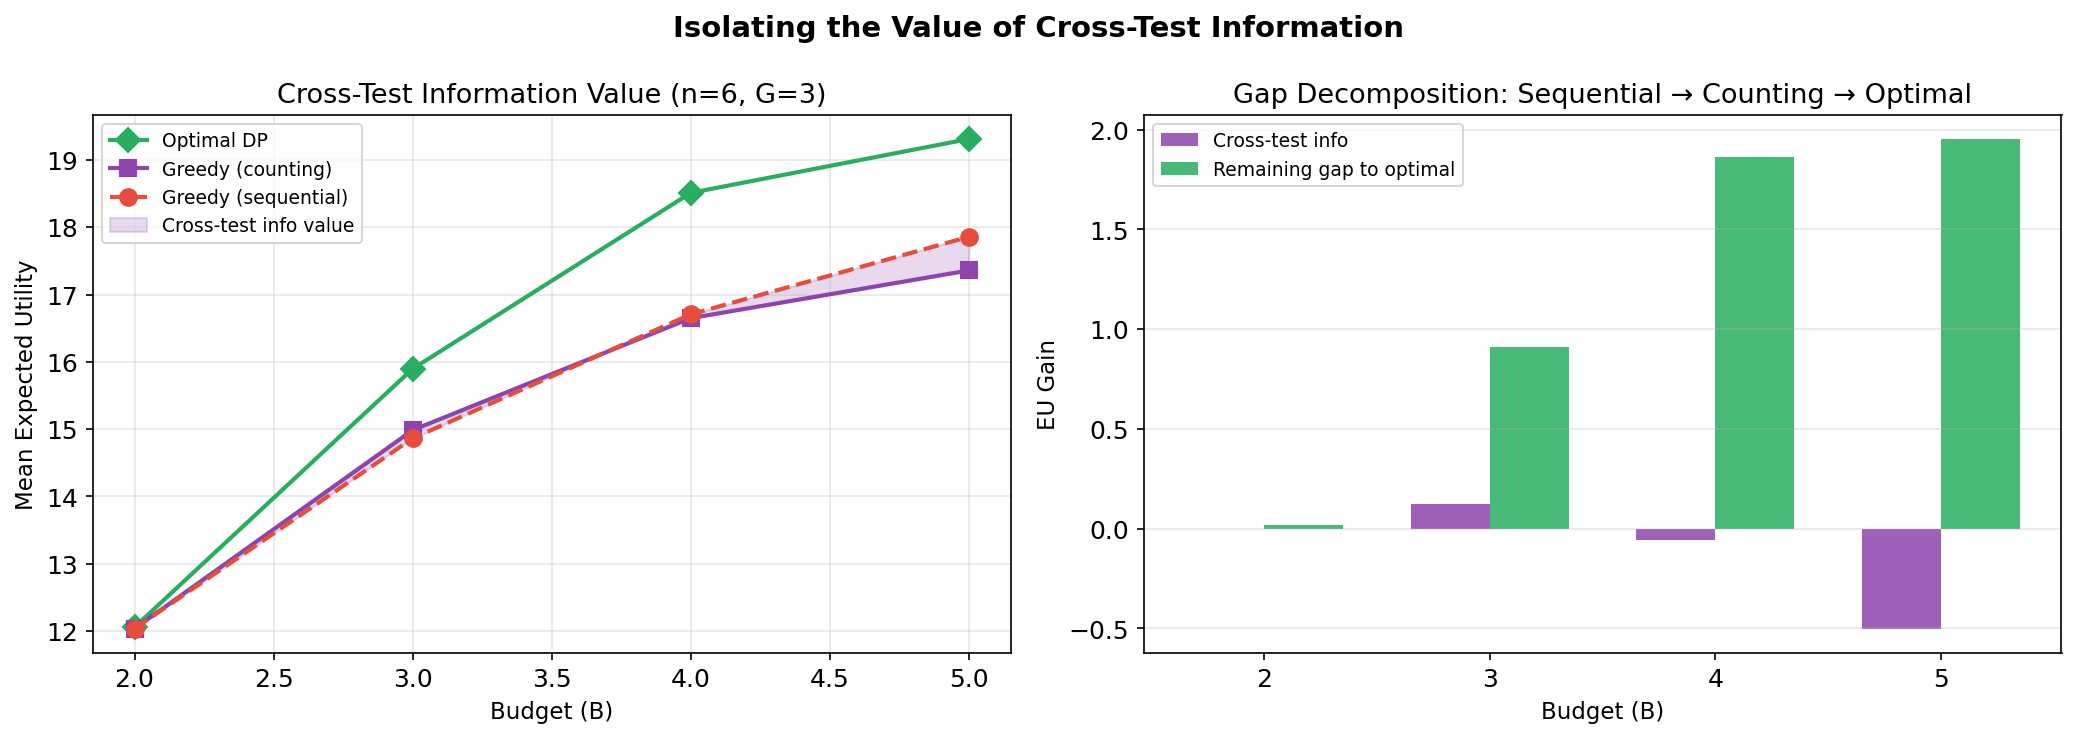
\includegraphics[width=0.7\textwidth]{cross_test_info_value.png}
  \caption{Valor de la informacion cruzada (counting $-$ secuencial). Mayor a $B$ intermedio, converge a $B$ grande.}
  \label{fig:crosstest}
\end{figure}

%% ====================================================================
\section{Que Tan Rapido es Cada Solver?}
\label{sec:scalability}

\textbf{Frontera de Pareto:} utilidad vs tiempo de computo para DP exacto, hibrido, y greedy ($n \in \{6, 8, 10\}$).

\textbf{Escalabilidad:} el DP exacto crece exponencialmente. Limite practico: $n \approx 10$--$11$.

\textbf{Cuando basta con greedy?} Heatmap del gap greedy-optimo por $(n, B)$.
Greedy es casi optimo para $B$ chico, pero el gap se amplía a $B$ mayor.

\begin{figure}[htbp]
  \centering
  \begin{subfigure}[t]{0.32\textwidth}
    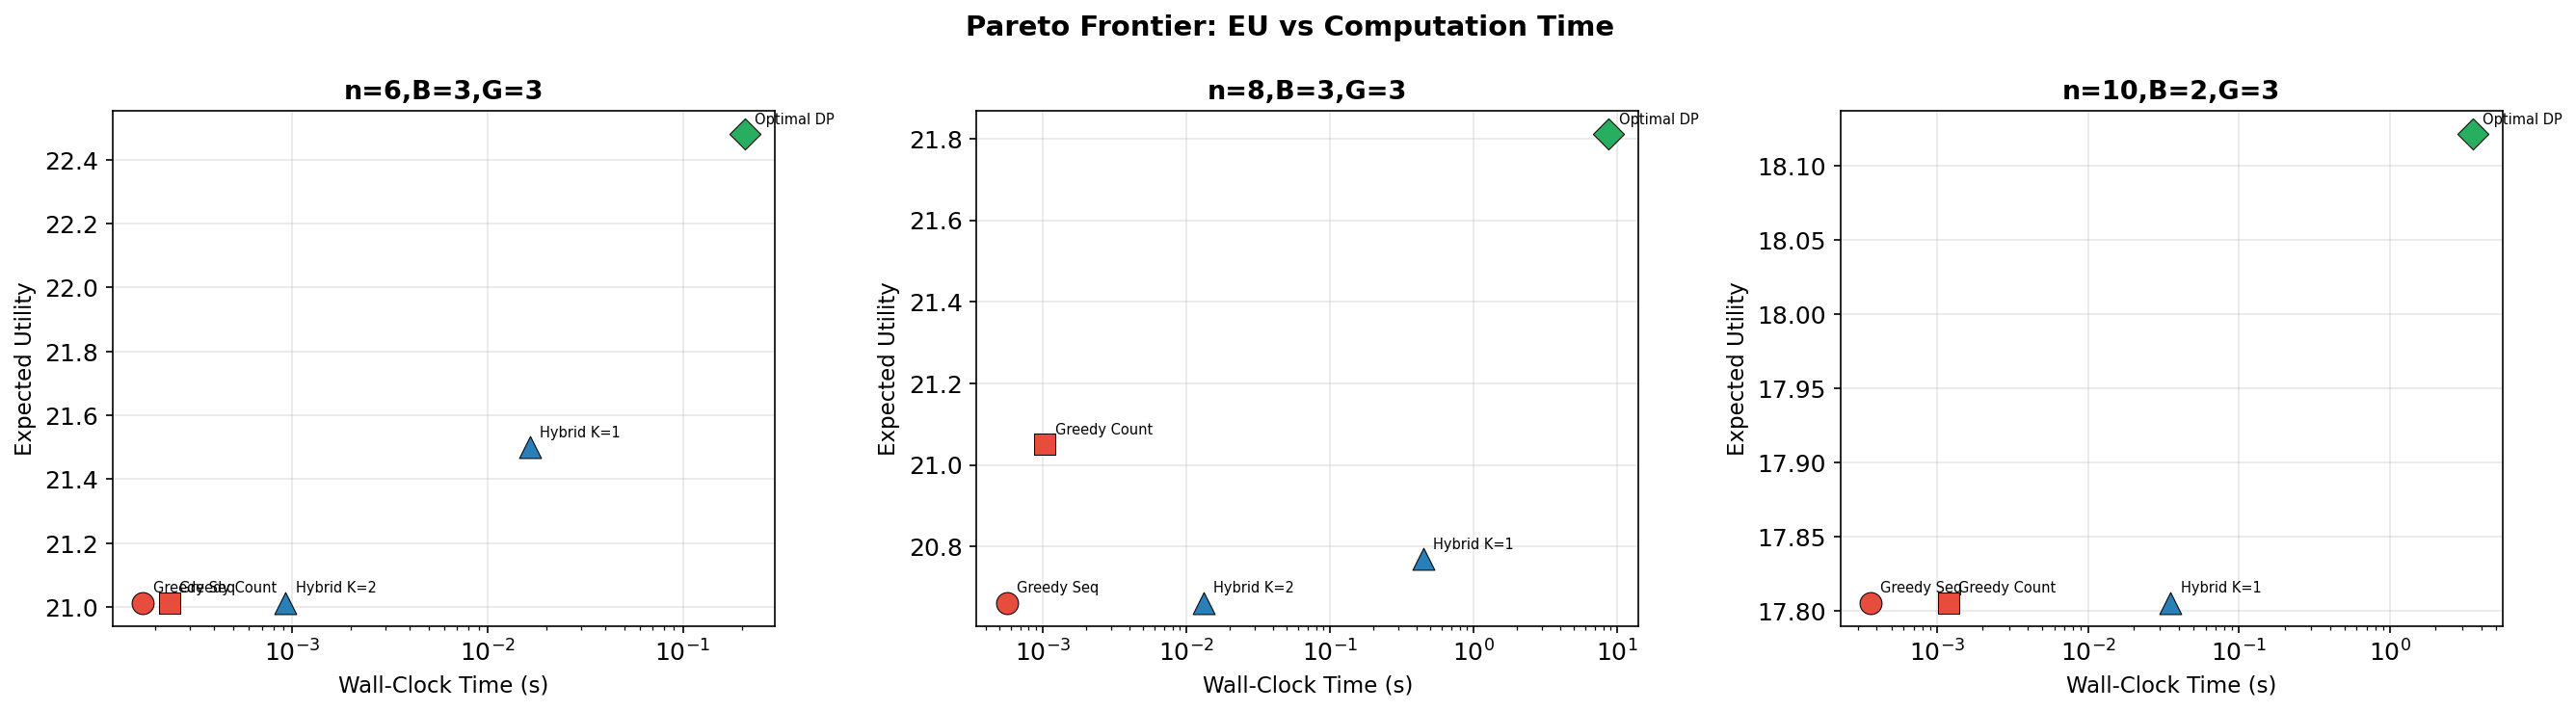
\includegraphics[width=\textwidth]{pareto_frontier.png}
    \caption{Pareto: EU vs tiempo.}
  \end{subfigure}
  \hfill
  \begin{subfigure}[t]{0.32\textwidth}
    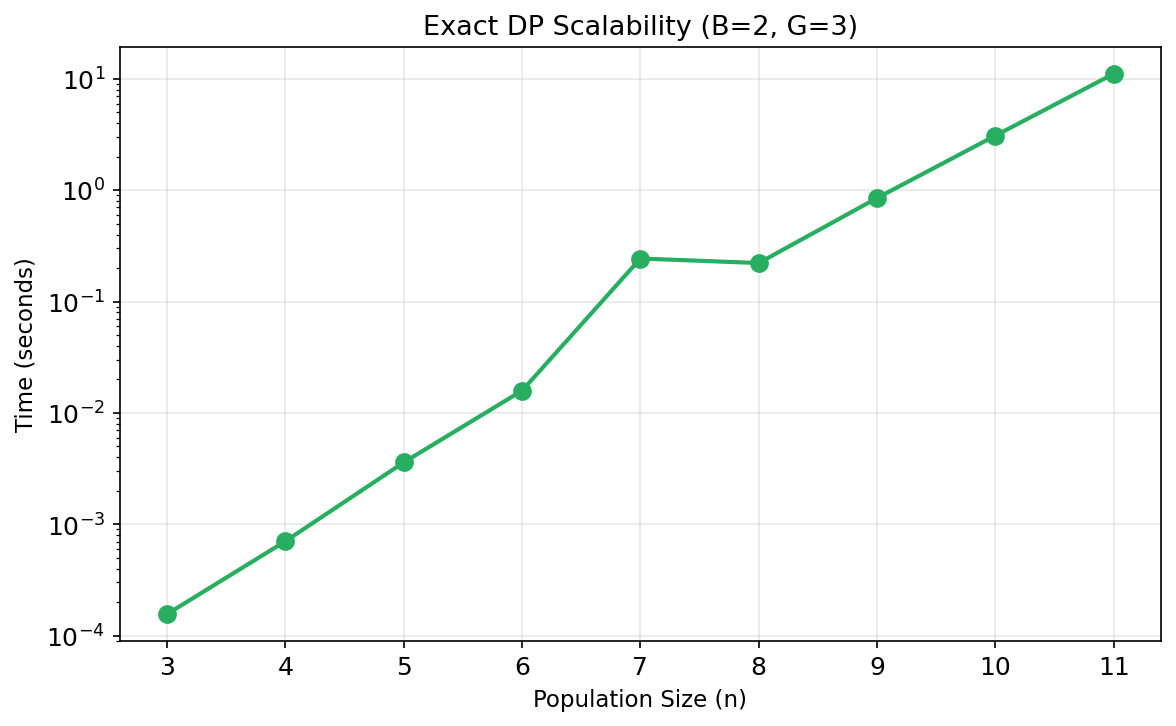
\includegraphics[width=\textwidth]{dp_scalability.png}
    \caption{Tiempo del DP vs $n$.}
  \end{subfigure}
  \hfill
  \begin{subfigure}[t]{0.32\textwidth}
    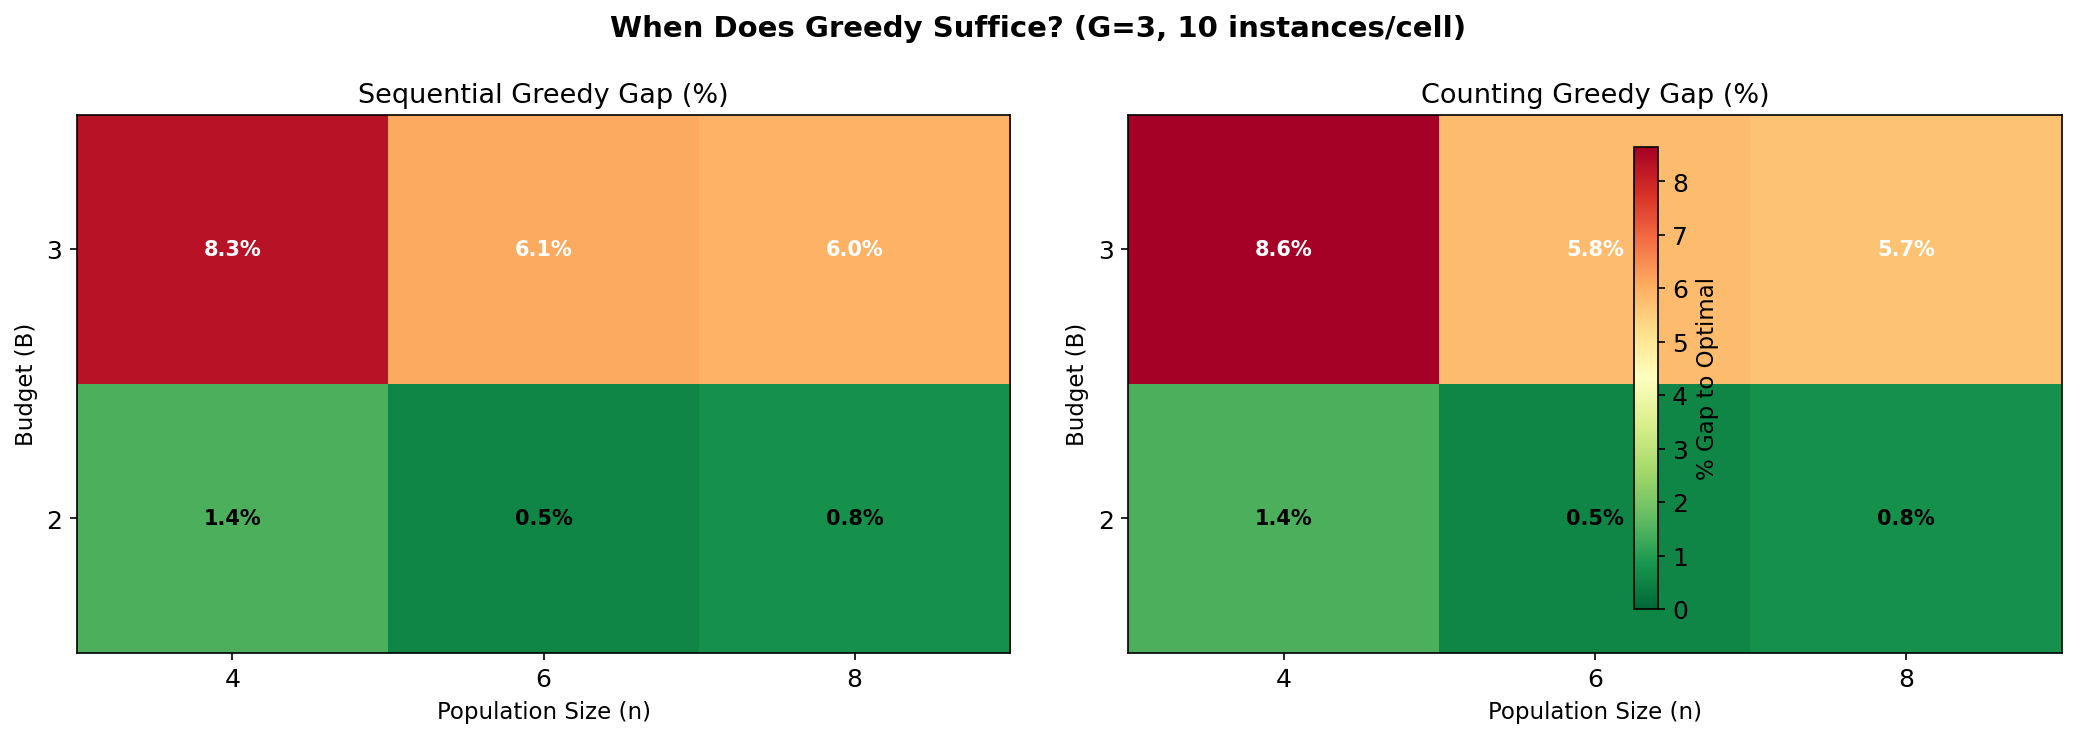
\includegraphics[width=\textwidth]{greedy_gap_heatmap.png}
    \caption{Gap greedy por $(n, B)$.}
  \end{subfigure}
  \caption{El DP es exacto pero lento. Greedy es rapido pero pierde calidad con $B$ grande.}
\end{figure}

%% ====================================================================
\section{Robustez: Que Pasa si las Probabilidades Estan Mal?}
\label{sec:robustness}

En la practica, no conocemos las $p_i$ exactas.

\textbf{Shift global:} optimizamos con $\hat{p}_i = p_i + \delta$, evaluamos con $p_i$ real.
El aumentado se compara contra un greedy clasico evaluado en $p_{\text{true}}$ como baseline.
Probado con $n=6$, $B=3$, $G=3$, 10 instancias.
Nota: el aumentado se evalua por Monte Carlo (200 sims/instancia), el clasico analiticamente.
Subestimar prevalencia ($\delta < 0$) duele mas que sobreestimar.

\textbf{Ruido individual:} agregamos ruido $N(0, \sigma)$ a cada $p_i$.
Con $\sigma = 0.20$, la utilidad baja poco.

\begin{figure}[htbp]
  \centering
  \begin{subfigure}[t]{0.48\textwidth}
    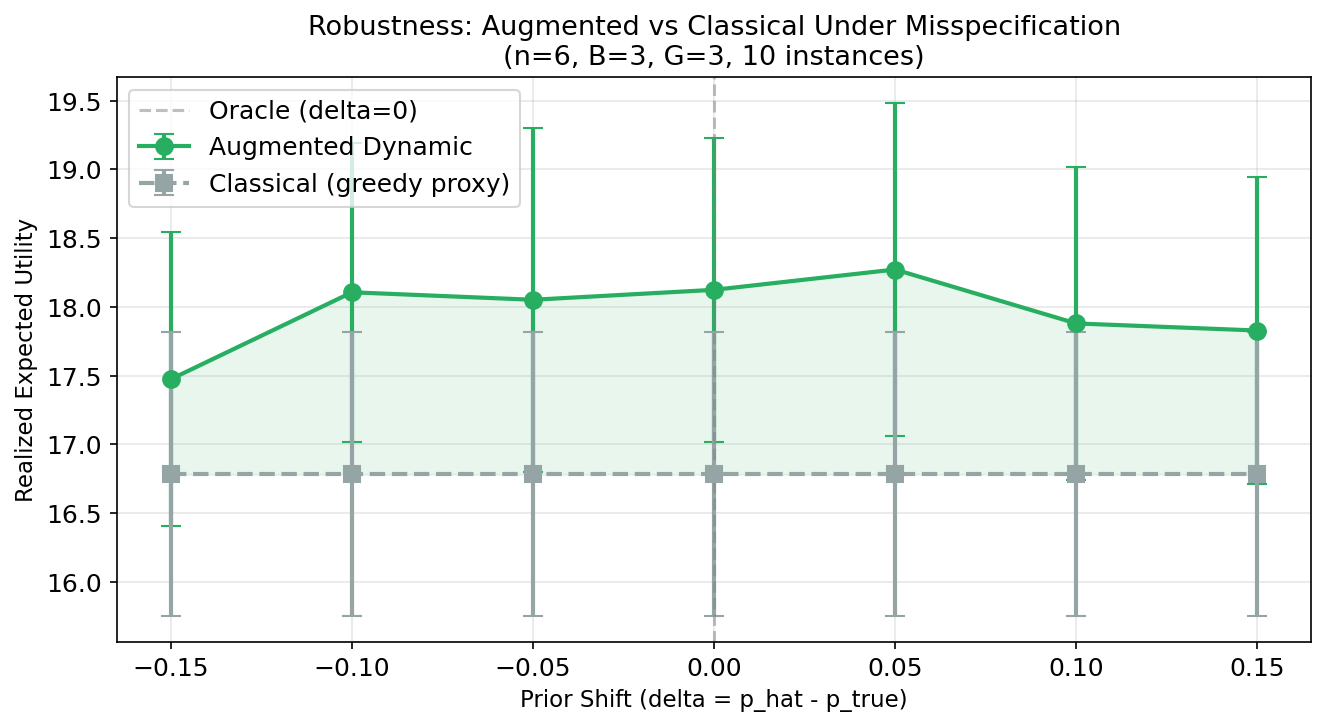
\includegraphics[width=\textwidth]{robustness_global_shift.png}
    \caption{Shift global: aumentado vs clasico.}
  \end{subfigure}
  \hfill
  \begin{subfigure}[t]{0.48\textwidth}
    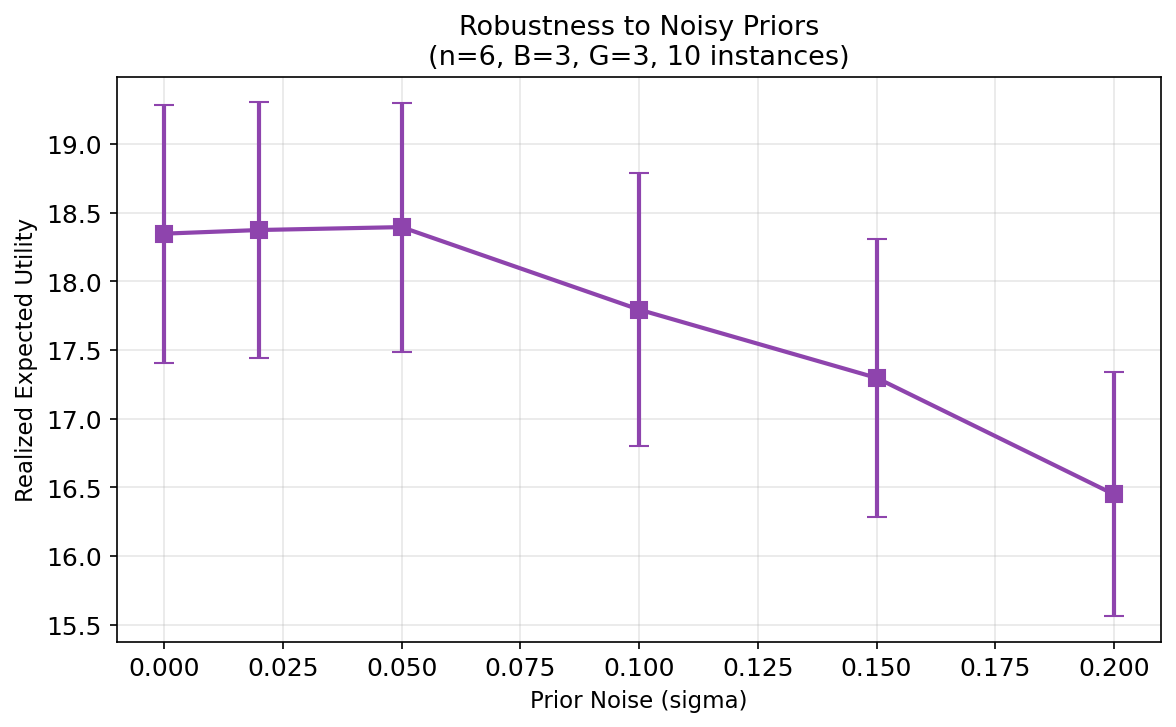
\includegraphics[width=\textwidth]{robustness_noisy_priors.png}
    \caption{Priors ruidosos.}
  \end{subfigure}
  \caption{La estrategia funciona bien aunque las probabilidades no sean exactas.}
\end{figure}

%% ====================================================================
\section{Riesgo: No Solo el Promedio}
\label{sec:risk}

El promedio no cuenta toda la historia. Tambien medimos:
\begin{itemize}
  \item $\Pr(\text{welfare} = 0)$: probabilidad de no aclarar a nadie
  \item $\text{CVaR}_{10}$: promedio del peor 10\% de casos
\end{itemize}

Con $n=5$, $B=2$, $G=3$, 10 instancias, 2000 simulaciones cada una.

El aumentado dinamico tiene el mejor promedio, pero el testeo individual puede tener menor P(welfare=0) en ciertos casos. Hay un trade-off entre utilidad esperada y riesgo de cola.

\begin{figure}[htbp]
  \centering
  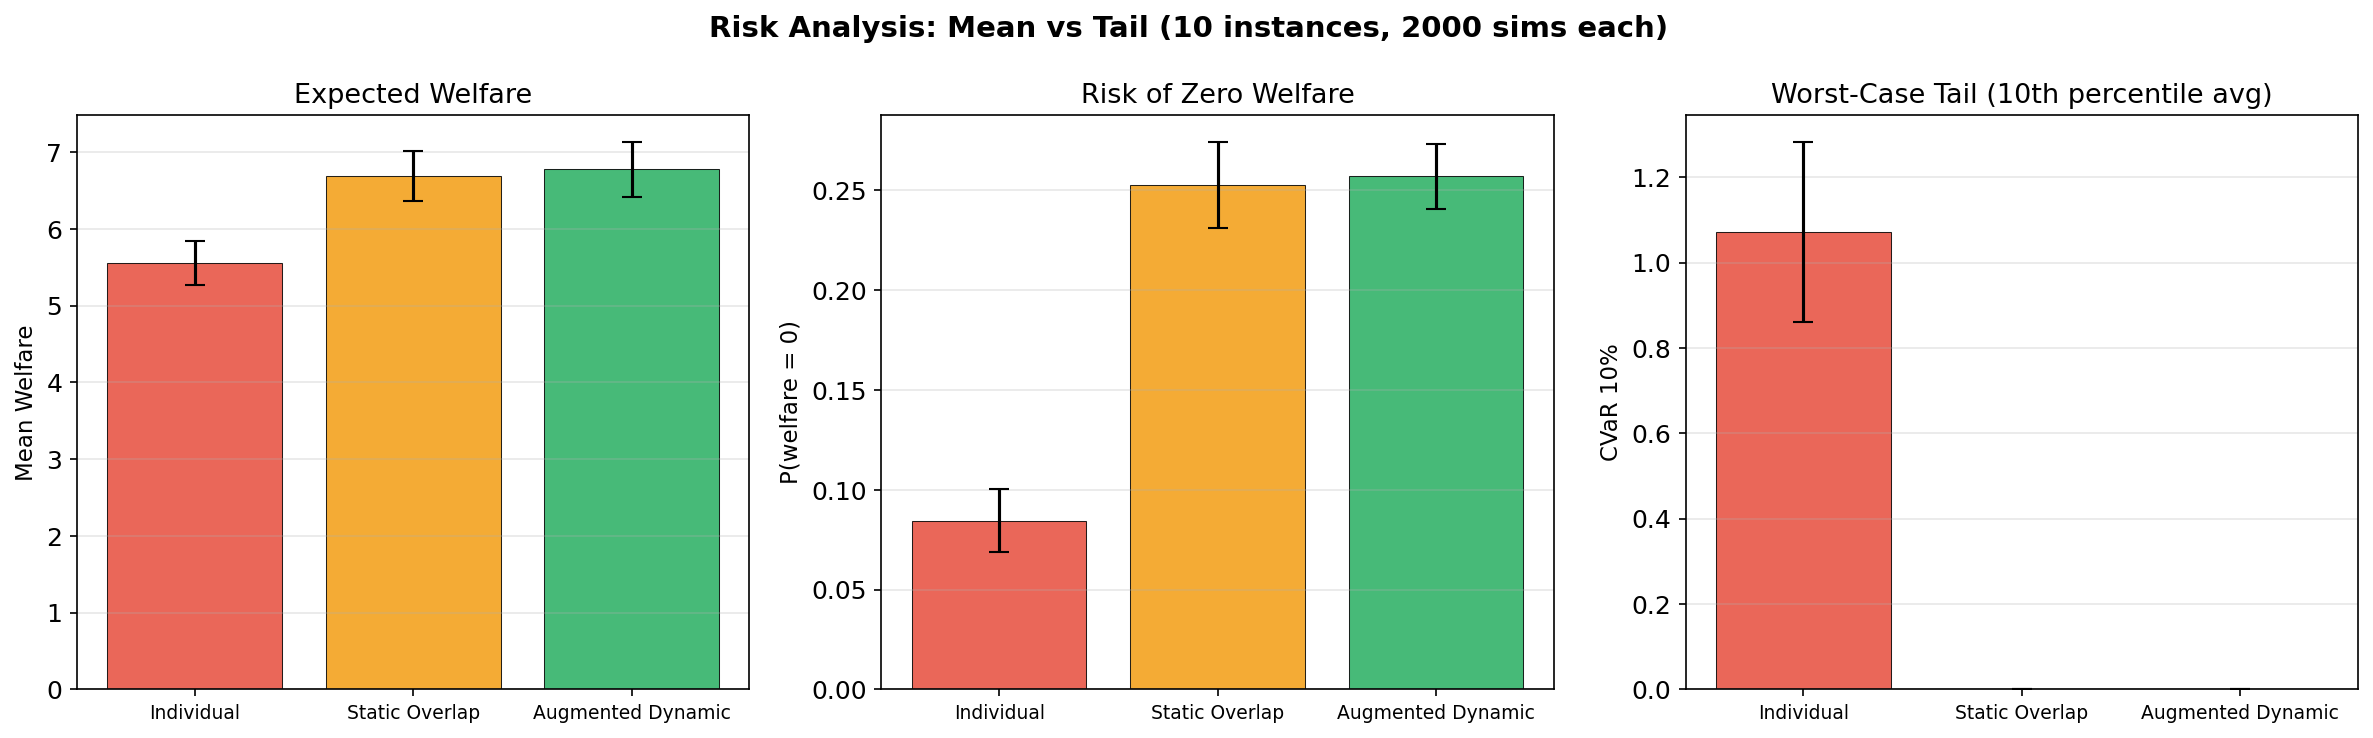
\includegraphics[width=0.75\textwidth]{risk_analysis.png}
  \caption{Promedio, riesgo de cero, y peor caso por estrategia.}
  \label{fig:risk}
\end{figure}

%% ====================================================================
\section{Escenarios Realistas}
\label{sec:scenarios}

5 escenarios motivados por aplicaciones reales:

\begin{table}[htbp]
  \centering
  \caption{Que pasa en cada escenario.}
  \begin{tabular}{lcp{7cm}}
    \toprule
    Escenario & Prevalencia & Que observamos \\
    \midrule
    Screening masivo & $\sim 2\%$ & Agrupar domina. Casi todos los grupos salen negativos. \\
    Cluster de exposicion & Moderada & Adaptarse y traslapar ayudan. \\
    Brote & $\sim 30\%$ & Adaptarse es clave. Hay que refinar los positivos. \\
    Brote severo & $\sim 80\%$ & Pocas ganancias. Casi todo sale positivo. \\
    Bimodal & Mixta & Aumentar ayuda mas. Los conteos distinguen subpoblaciones. \\
    \bottomrule
  \end{tabular}
\end{table}

\begin{figure}[htbp]
  \centering
  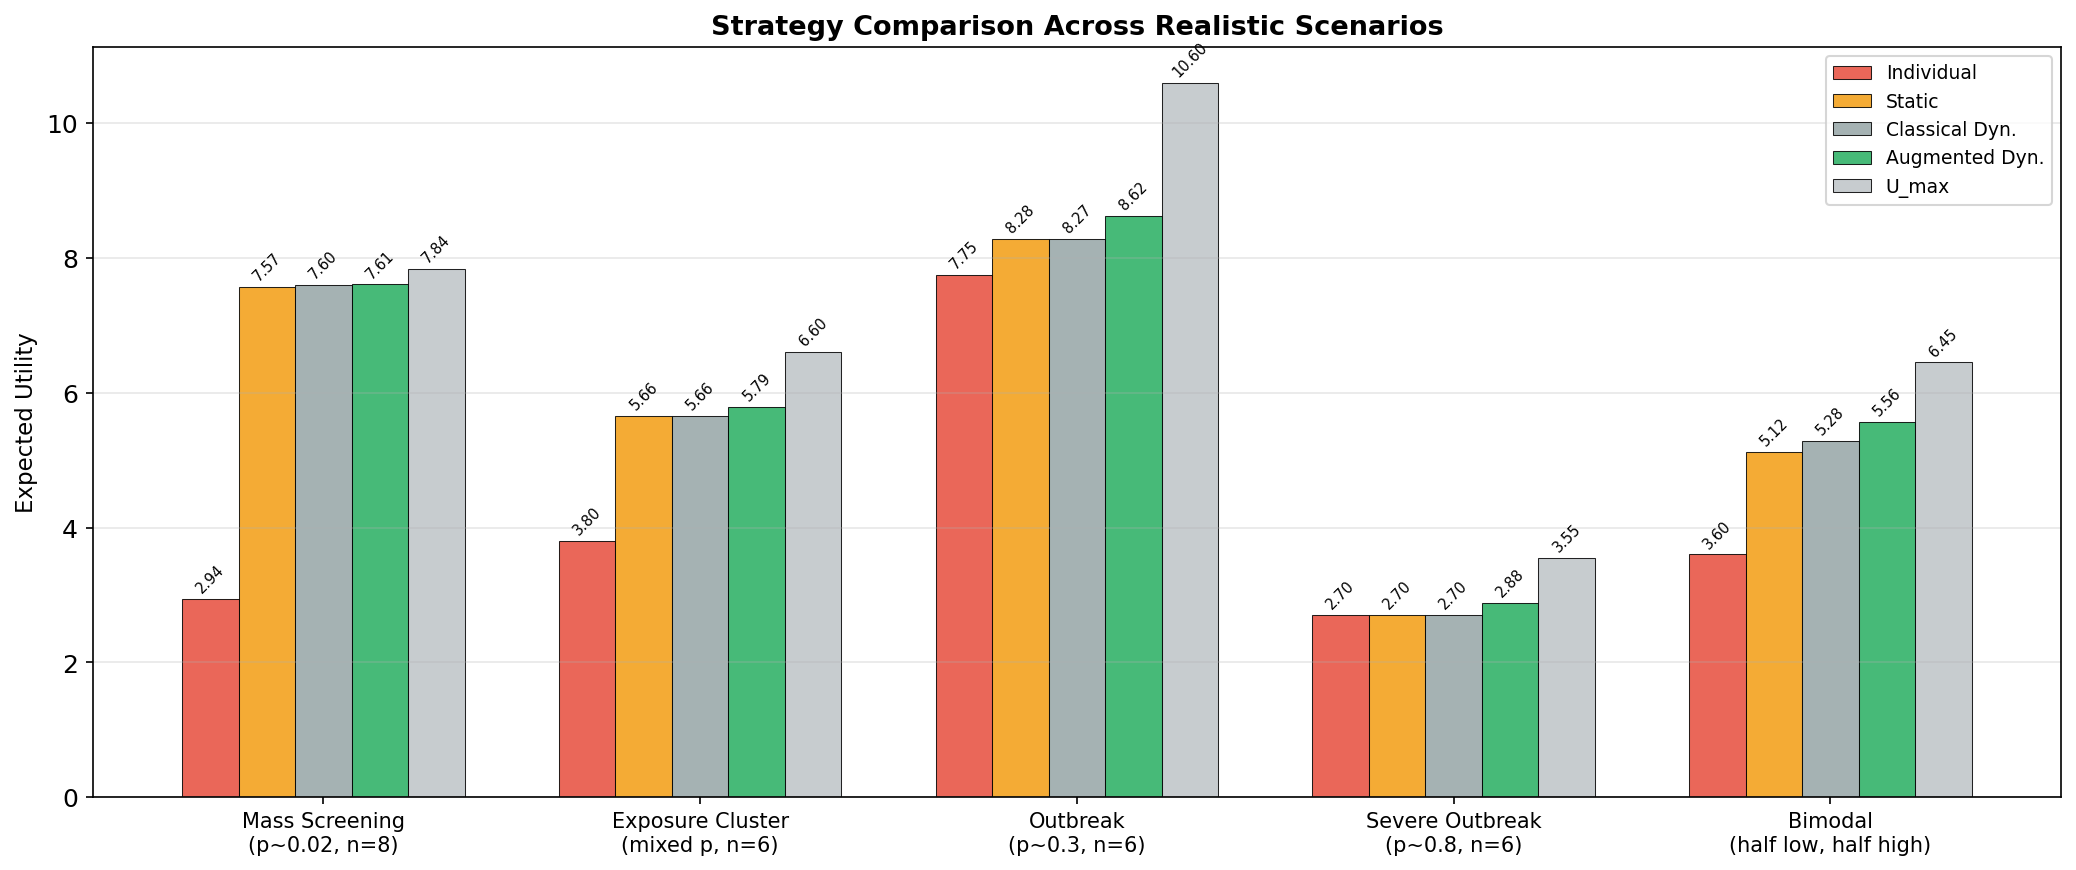
\includegraphics[width=0.85\textwidth]{realistic_scenarios.png}
  \caption{Comparacion de estrategias en 5 escenarios.}
\end{figure}

%% ====================================================================
\section*{Apendices}

Verificaciones adicionales en el notebook:

\begin{description}
  \item[Gibbs] El muestreador converge correctamente (Fig.~\ref{fig:app-gibbs}).
  \item[Hibrido] Barrido de $K$ pasos greedy antes de DP (Fig.~\ref{fig:app-hybrid}).
  \item[Alpha/Beta] Efecto de parametros de scoring (Figs.~\ref{fig:app-alpha},~\ref{fig:app-beta}).
  \item[Tesis Nico] Replicacion de ejemplos 4.4 y escalamiento (Figs.~\ref{fig:app-nico},~\ref{fig:app-budget}).
\end{description}

\begin{figure}[htbp]
  \centering
  \begin{subfigure}[t]{0.32\textwidth}
    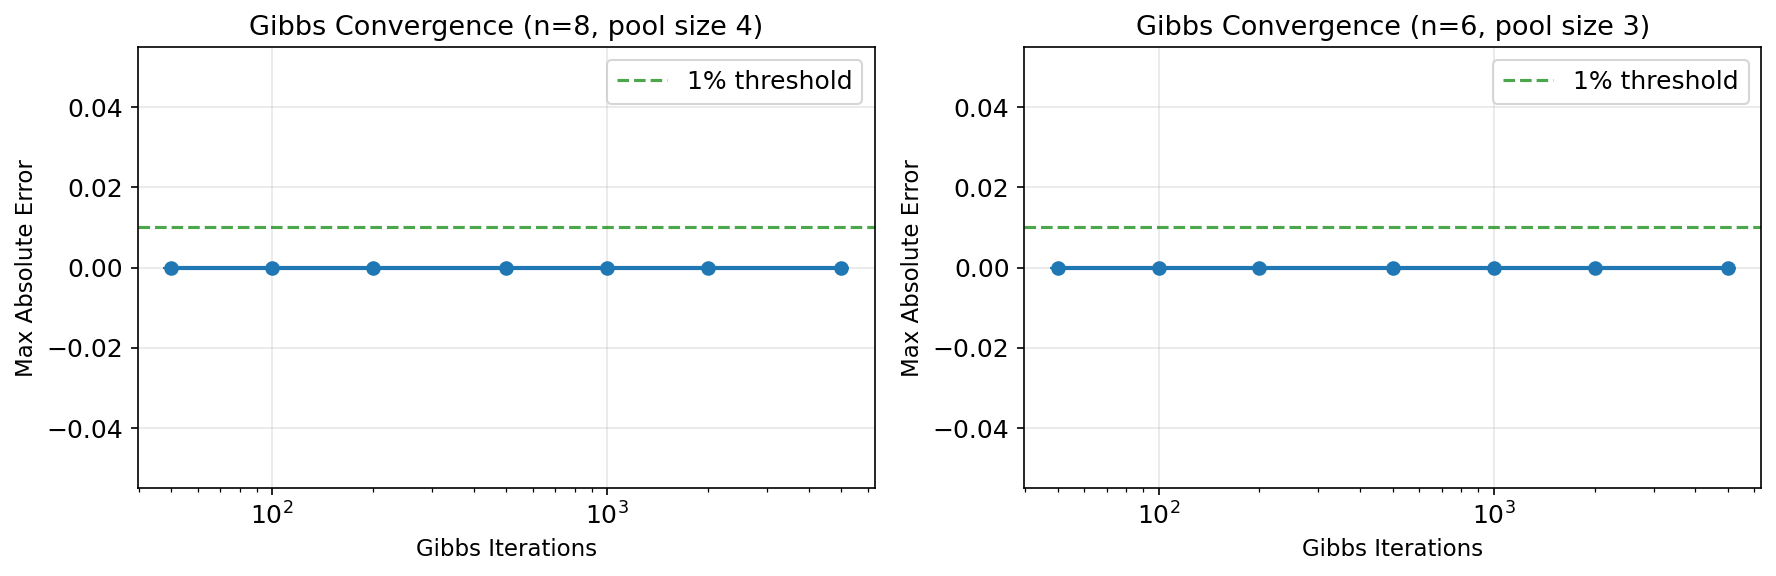
\includegraphics[width=\textwidth]{appendix_gibbs_convergence.png}
    \caption{Gibbs.}
    \label{fig:app-gibbs}
  \end{subfigure}
  \hfill
  \begin{subfigure}[t]{0.32\textwidth}
    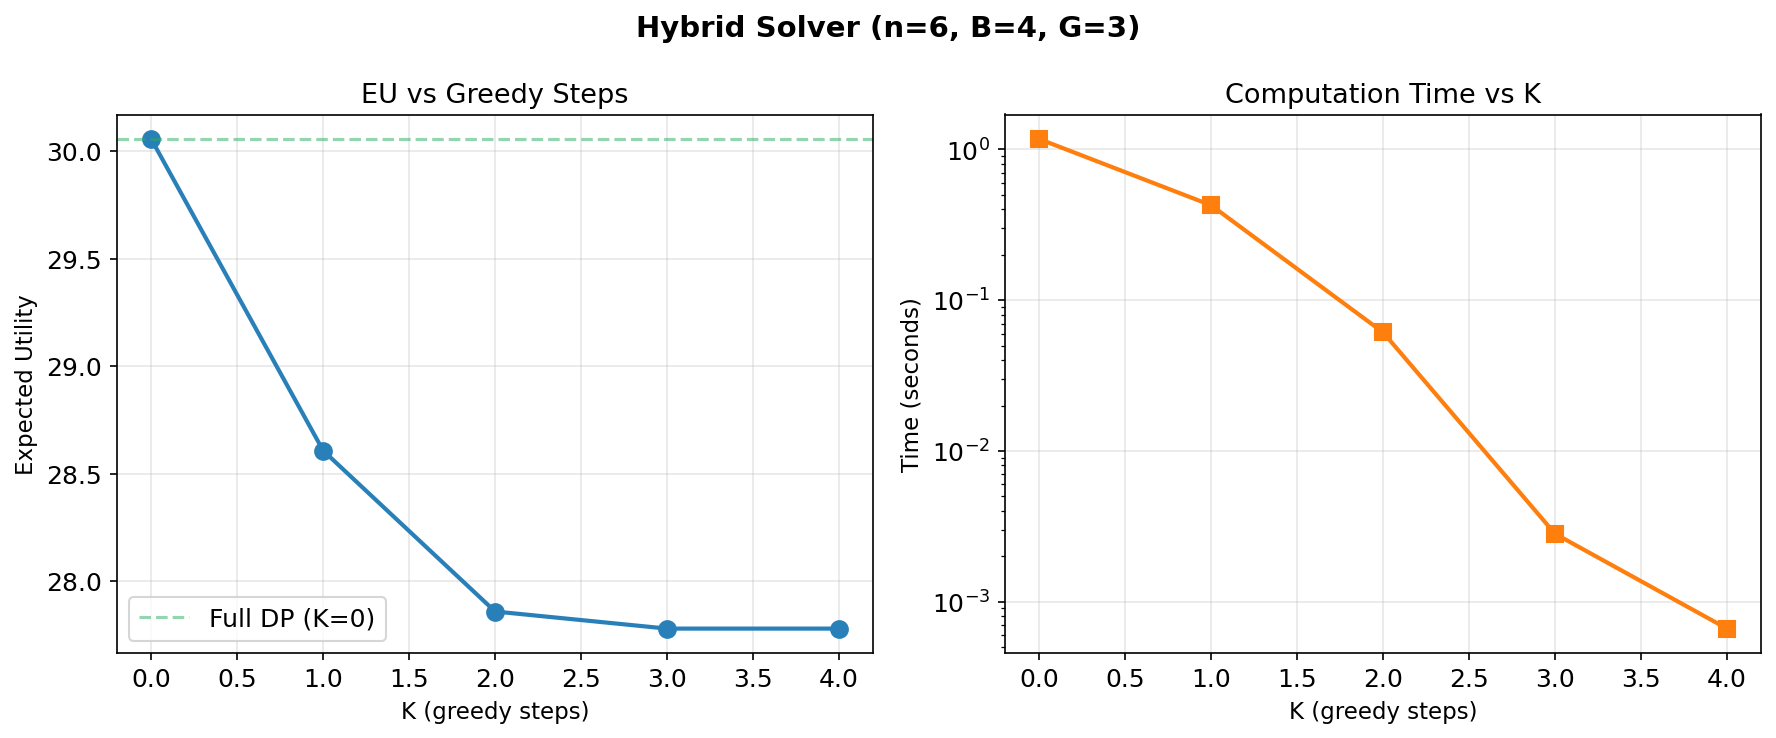
\includegraphics[width=\textwidth]{appendix_hybrid_sweep.png}
    \caption{Hibrido $K$.}
    \label{fig:app-hybrid}
  \end{subfigure}
  \hfill
  \begin{subfigure}[t]{0.32\textwidth}
    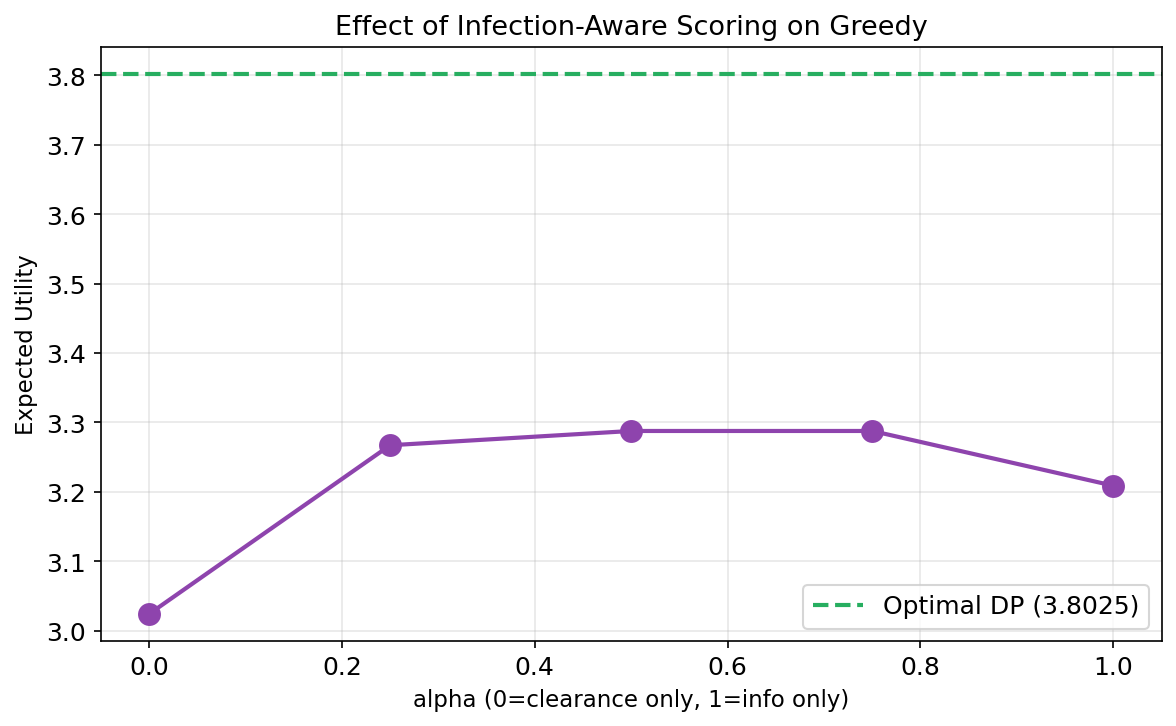
\includegraphics[width=\textwidth]{appendix_alpha_sweep.png}
    \caption{Alpha.}
    \label{fig:app-alpha}
  \end{subfigure}
\end{figure}

\begin{figure}[htbp]
  \centering
  \begin{subfigure}[t]{0.32\textwidth}
    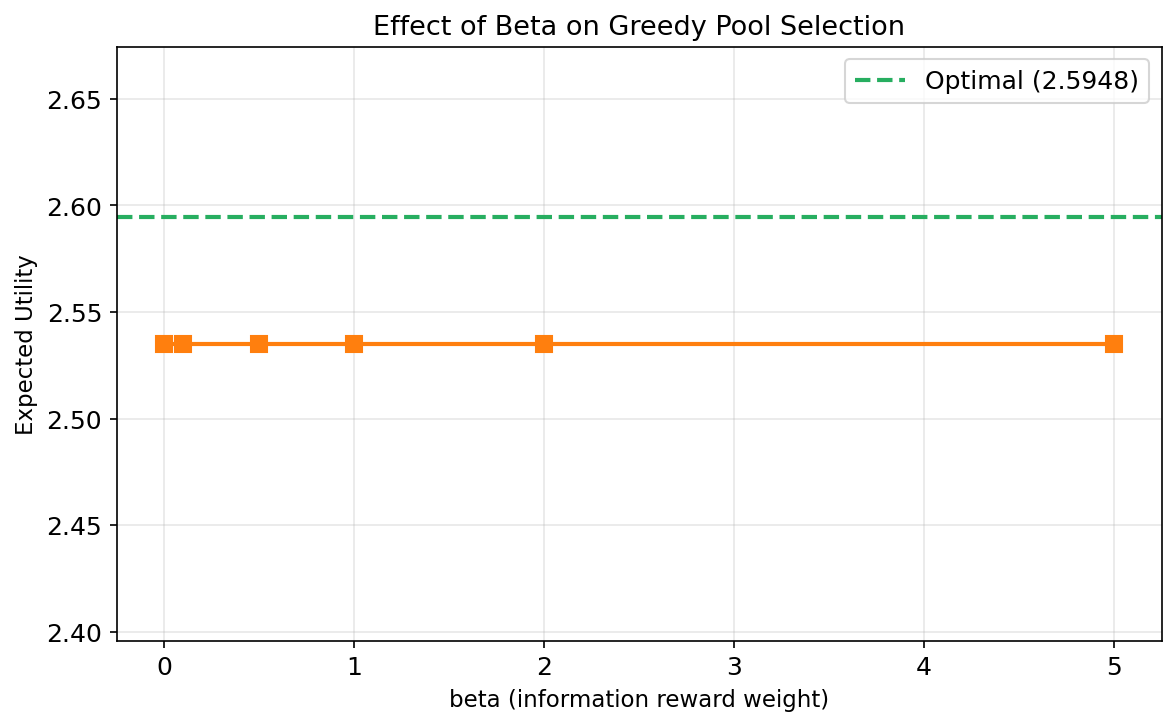
\includegraphics[width=\textwidth]{appendix_beta_sweep.png}
    \caption{Beta.}
    \label{fig:app-beta}
  \end{subfigure}
  \hfill
  \begin{subfigure}[t]{0.32\textwidth}
    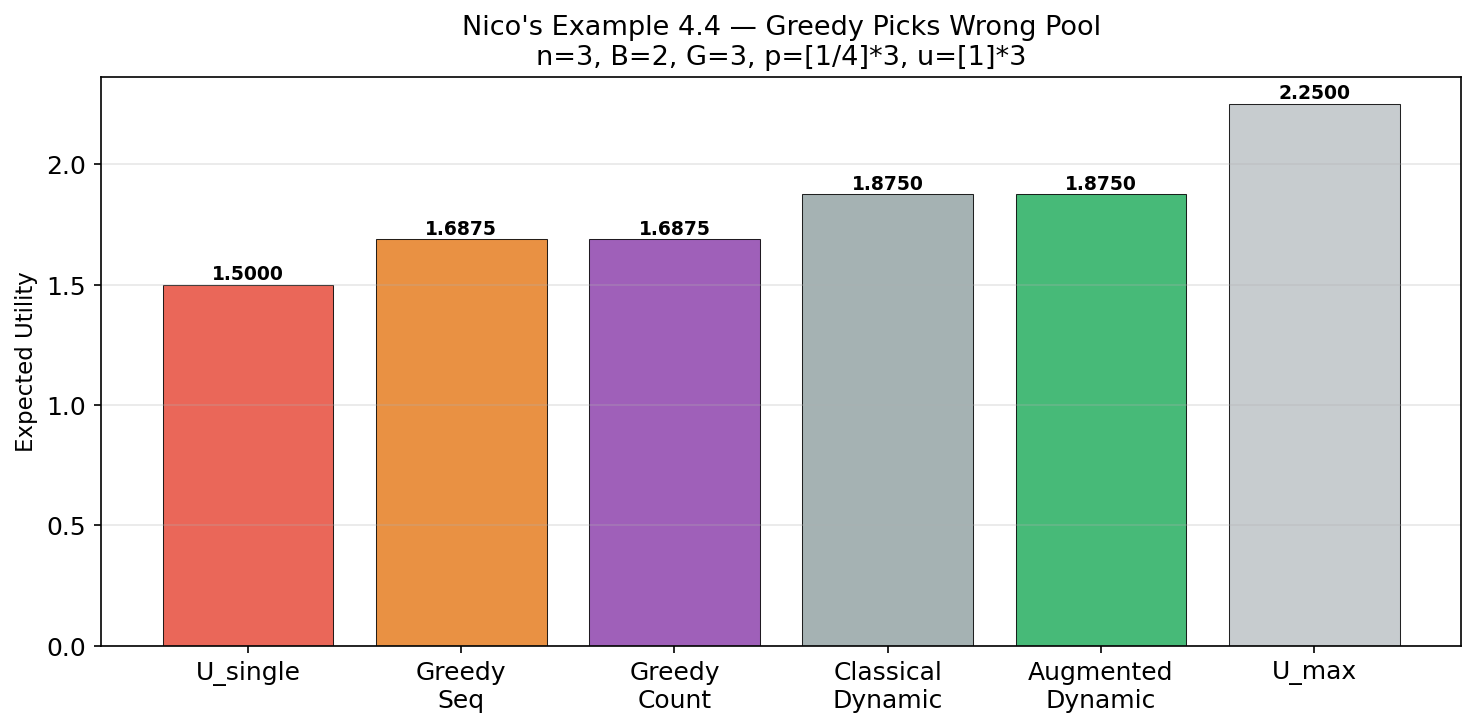
\includegraphics[width=\textwidth]{appendix_nico_ex44.png}
    \caption{Nico Ej. 4.4.}
    \label{fig:app-nico}
  \end{subfigure}
  \hfill
  \begin{subfigure}[t]{0.32\textwidth}
    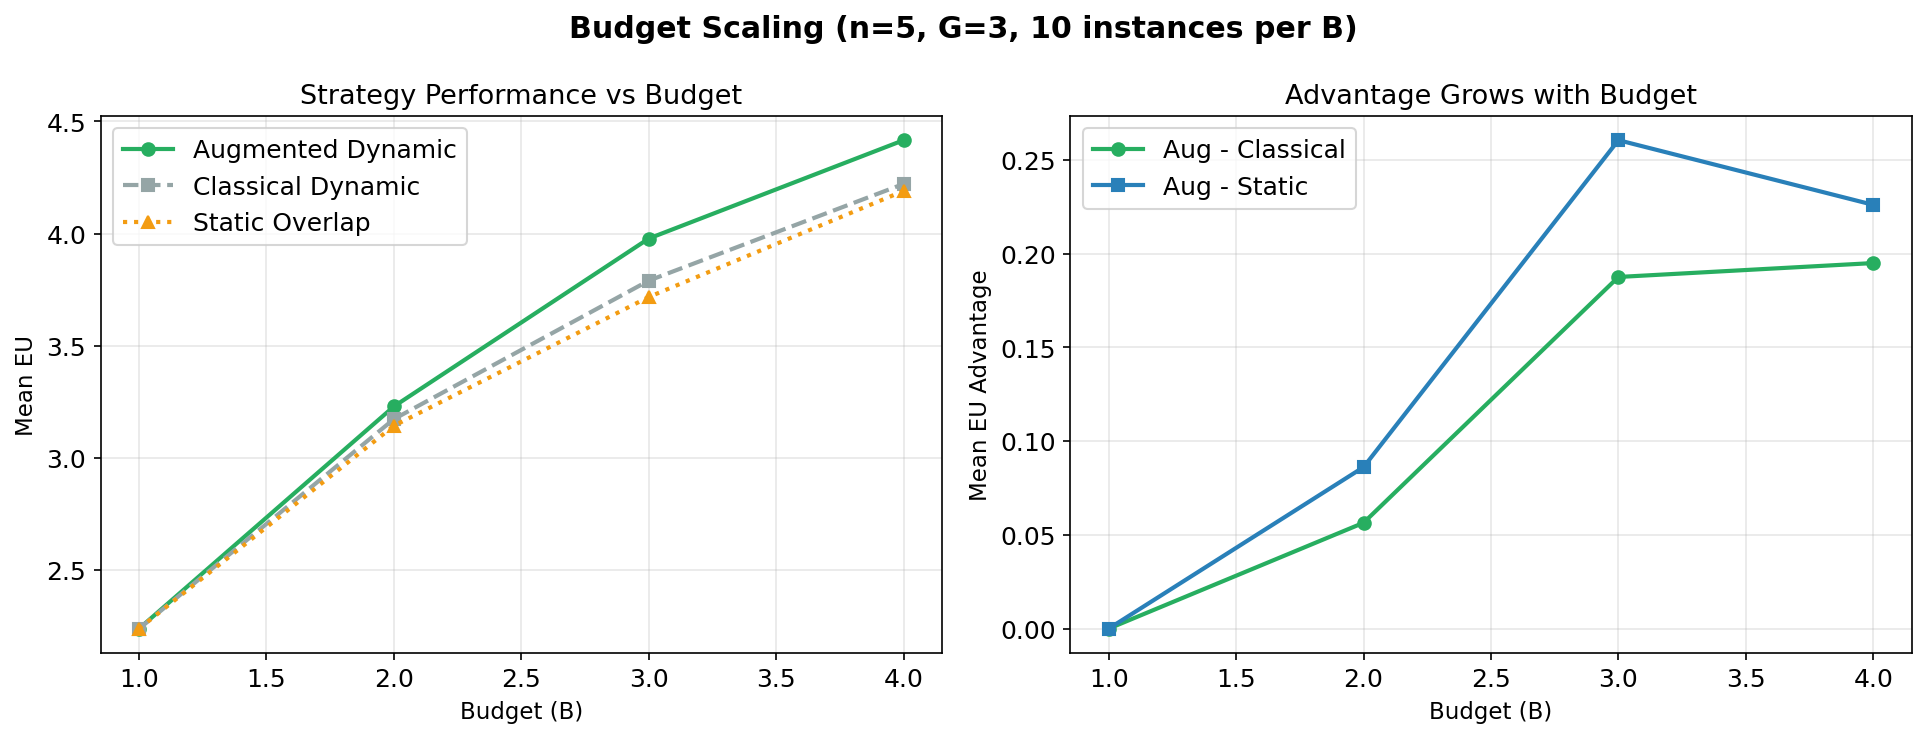
\includegraphics[width=\textwidth]{appendix_budget_scaling.png}
    \caption{Escalamiento $B$.}
    \label{fig:app-budget}
  \end{subfigure}
  \caption{Apendices.}
\end{figure}

\end{document}
